\chapter{\difficult{Higher-dimensional Algebra}}\label{chapter:hda}

    The main reference for this chapter is a series of eponymous papers~\citep{baez_higher-dimensional_2003, baez_higher-dimensional_2003-1}. For Kapranov-Voevodsky 2-vector spaces, the reader is referred to the original paper by~\citet{kapranov_2-categories_1994}. References for the section on Berezin calculus are~\citet{losev_berezin_2007, choquet-bruhat_analysis_2000}. The section about higher Lie theory is mainly based on~\citet{fiorenza_introduction_2004}. For fusion and modular categories, the main reference is~\citet{etingof_tensor_2016}.

    \minitoc

\section{Monoidal categories}\label{section:monoidal_categories}

    \newdef{Monoidal category}{\index{monoidal!category}\index{tensor product}\label{cat:monoidal_category}
        A category $\symbfsf{C}$ equipped with a bifunctor
        \begin{gather}
            -\otimes -:\symbfsf{C}\times\symbfsf{C}\rightarrow\symbfsf{C}\,,
        \end{gather}
        called the \textbf{tensor product} or \textbf{monoidal product}, a distinct object $\symbf{1}$, called the \textbf{(monoidal) unit}, and the following three natural isomorphisms, called the \textbf{coherence maps}:
        \begin{itemize}
            \item\textbf{Associator}: $\alpha_{x,y,z}:(x\otimes y)\otimes z\cong x\otimes(y\otimes z)$,
            \item\textbf{Left unitor}: $\lambda_x:\symbf{1}\otimes x\cong x$, and
            \item\textbf{Right unitor}: $\rho_x:x\otimes\symbf{1}\cong x$.
        \end{itemize}
        These natural transformations are required make the \textbf{triangle} and \textbf{pentagon} diagrams in \cref{fig:triangle_diagram} and \cref{fig:pentagon_diagram}, respectively, commute. A monoidal category for which the associator and the unitors are identity transformations is often said to be \textbf{strict}.

        \begin{figure}[ht!]
            \centering
            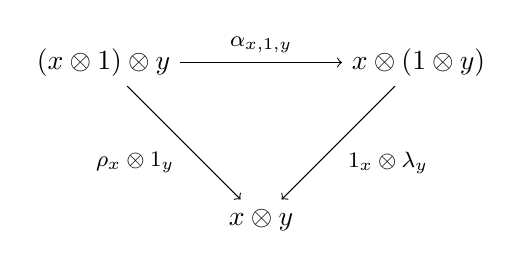
\begin{tikzpicture}
                \node (1) at (0, 0) {$(x\otimes\symbf{1})\otimes y$};
                \node (2) at (4, 0) {$x\otimes(\symbf{1}\otimes y)$};
                \node (3) at (2, -2) {$x\otimes y$};
                \draw[->] (1) -- node[above]{\footnotesize$\alpha_{x,\symbf{1},y}$} (2);
                \draw[->] (1) -- node[below left]{\footnotesize$\rho_x\otimes\mathbbm{1}_y$} (3);
                \draw[->] (2) -- node[below right]{\footnotesize$\mathbbm{1}_x\otimes\lambda_y$} (3);
            \end{tikzpicture}
            \caption{Triangle diagram.}
            \label{fig:triangle_diagram}
        \end{figure}
    }

    \begin{figure}[ht!]
        \centering
        \begin{tikzpicture}
            \node (1) at (0, 0) {$\bigl((w\otimes x)\otimes y\bigr)\otimes z$};
            \node (2) at (6, 0) {$\bigl(w\otimes(x\otimes y)\bigr)\otimes z$};
            \node (3) at (-2, -3) {$(w\otimes x)\otimes(y\otimes z)$};
            \node (4) at (8, -3) {$w\otimes\bigl((x\otimes y)\otimes z\bigr)$};
            \node (5) at (3, -6) {$w\otimes\bigl(x\otimes(y\otimes z)\bigr)$};
            \draw[->] (1) -- node[above]{\small$\alpha_{w,x,y}\otimes\mathbbm{1}_z$} (2);
            \draw[->] (1) -- node[above left]{\small$\alpha_{w\otimes x,y,z}$} (3);
            \draw[->] (3) -- node[below left]{\small$\alpha_{w,x,y\otimes z}$} (5);
            \draw[->] (2) -- node[above right]{\small$\alpha_{w,x\otimes y,z}$} (4);
            \draw[->] (4) -- node[below right]{\small$\mathbbm{1}_w\otimes\alpha_{x,y,z}$} (5);
        \end{tikzpicture}
        \caption{Pentagon diagram.}
        \label{fig:pentagon_diagram}
    \end{figure}

    \begin{example}[Cartesian category]\label{cat:semicartesian}
        A monoidal category where the monoidal product is given by the ordinary product (\cref{cat:product}). If the monoidal product is not the ordinary product, but the monoidal unit is still terminal, the category is said to be \textbf{semicartesian}.
    \end{example}

    \newdef{Scalar}{\index{scalar}
        In a monoidal category, the scalars are defined as the endomorphisms $\symbf{1}\rightarrow\symbf{1}$. The set of scalars forms a commutative monoid.
    }
    \begin{property}
        Every scalar $s:\symbf{1}\rightarrow\symbf{1}$ induces a natural transformation $s:\mathbbm{1}_{\symbfsf{C}}\Rightarrow\mathbbm{1}_{\symbfsf{C}}$ with components
        \begin{gather}
            s_x:x\cong\symbf{1}\otimes x\overset{s\otimes\mathbbm{1}_x}{\longrightarrow}\symbf{1}\otimes x\cong x\,.
        \end{gather}
        For every morphism $f\in\mathrm{hom}(\symbfsf{C})$, the naturality square $f\circ s_x=s_y\circ f$ alo defines a morphism $s\diamond f$ that is equivalently given by $\rho_y\circ(f\otimes s)\circ\rho^{-1}_x$ (one could have used the left unitors as well). These morphisms satisfy the following well-known rules of scalar multiplication from linear algebra:
        \begin{itemize}
            \item $s\diamond(s'\diamond f) = (s\circ s')\diamond f$,
            \item $(s\diamond f)\circ(s'\diamond g) = (s\circ s')\diamond(f\circ g)$, and
            \item $(s\diamond f)\otimes(s'\diamond g) = (s\circ s')\diamond(f\otimes g)$.
        \end{itemize}
    \end{property}

    \newdef{Weak inverse}{\index{weak!inverse}
        Let $(\symbfsf{C},\otimes,\symbf{1})$ be a monoidal category. An object $y\in\ob{C}$ is called a weak inverse of an object $x\in\ob{C}$ if it satisfies $x\otimes y\cong\symbf{1}$.
    }
    \begin{remark}
        One can show that the existence of a one-sided weak inverse (as in the definition above) implies that it is in fact a two-sided weak inverse, i.e.~$y\otimes x\cong\symbf{1}$ also holds.
    \end{remark}

    \begin{theorem}[MacLane's coherence theorem]\index{MacLane!coherence theorem}\index{coherence|seealso{MacLane}}
        Consider two functors $\func{F,G}{A}{B}$ between two monoidal categories $\symbfsf{A},\symbfsf{B}$. Any two natural transformations $\eta,\varepsilon:F\Rightarrow G$, constructed solely from the associator and the unitors, coincide.
    \end{theorem}

\subsection{Braided categories}

    \newdef{Braided monoidal category}{\index{braiding}
        A monoidal category $(\symbfsf{C},\otimes,\symbf{1})$ equipped with a natural isomorphism
        \begin{gather}
            \sigma_{x,y}:x\otimes y\cong y\otimes x
        \end{gather}
        that makes the two \textbf{hexagon} diagrams~\ref{fig:hexagon_diagrams1} and~\ref{fig:hexagon_diagrams2} commute for all $x,y,z\in\ob{C}$. The isomorphism $\sigma$ is called the \textbf{braiding} (morphism).
        \begin{figure}[ht!]
            \centering
            \begin{subfigure}[b]{0.49\textwidth}
                \centering
                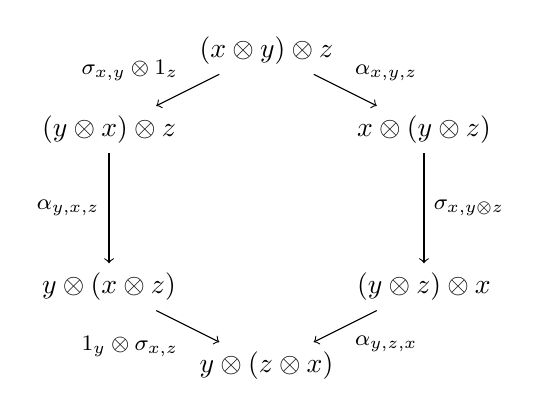
\begin{tikzpicture}
                    \node (1) at (0, 0) {$(x\otimes y)\otimes z$};
                    \node (2) at (-2, -1) {$(y\otimes x)\otimes z$};
                    \node (3) at (2, -1) {$x\otimes(y\otimes z)$};
                    \node (4) at (-2, -3) {$y\otimes(x\otimes z)$};
                    \node (5) at (2, -3) {$(y\otimes z)\otimes x$};
                    \node (6) at (0, -4) {$y\otimes(z\otimes x)$};
                    \draw[->] (1) -- node[above left]{\footnotesize$\sigma_{x,y}\otimes\mathbbm{1}_z$} (2);
                    \draw[->] (1) -- node[above right]{\footnotesize$\alpha_{x,y,z}$} (3);
                    \draw[->] (2) -- node[left]{\footnotesize$\alpha_{y,x,z}$} (4);
                    \draw[->] (3) -- node[right]{\footnotesize$\sigma_{x,y\otimes z}$} (5);
                    \draw[->] (4) -- node[below left]{\footnotesize$\mathbbm{1}_y\otimes\sigma_{x,z}$} (6);
                    \draw[->] (5) -- node[below right]{\footnotesize$\alpha_{y,z,x}$} (6);
                \end{tikzpicture}
                \caption{Hexagon diagram 1.}
                \label{fig:hexagon_diagrams1}
            \end{subfigure}
            \begin{subfigure}[b]{0.49\textwidth}
                \centering
                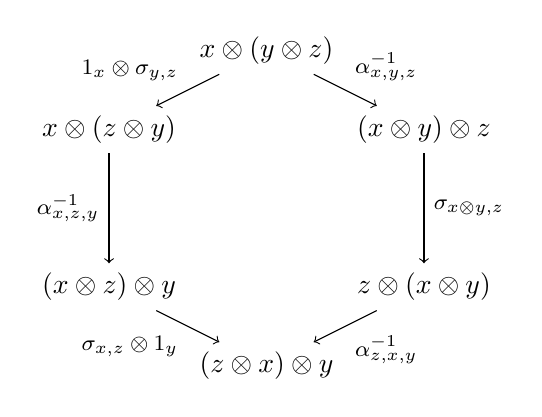
\begin{tikzpicture}
                    \node (1) at (0, 0) {$x\otimes(y\otimes z)$};
                    \node (2) at (-2, -1) {$x\otimes(z\otimes y)$};
                    \node (3) at (2, -1) {$(x\otimes y)\otimes z$};
                    \node (4) at (-2, -3) {$(x\otimes z)\otimes y$};
                    \node (5) at (2, -3) {$z\otimes(x\otimes y)$};
                    \node (6) at (0, -4) {$(z\otimes x)\otimes y$};
                    \draw[->] (1) -- node[above left]{\footnotesize$\mathbbm{1}_x\otimes\sigma_{y,z}$} (2);
                    \draw[->] (1) -- node[above right]{\footnotesize$\alpha^{-1}_{x,y,z}$} (3);
                    \draw[->] (2) -- node[left]{\footnotesize$\alpha^{-1}_{x,z,y}$} (4);
                    \draw[->] (3) -- node[right]{\footnotesize$\sigma_{x\otimes y,z}$} (5);
                    \draw[->] (4) -- node[below left]{\footnotesize$\sigma_{x,z}\otimes\mathbbm{1}_y$} (6);
                    \draw[->] (5) -- node[below right]{\footnotesize$\alpha^{-1}_{z,x,y}$} (6);
                \end{tikzpicture}
                \caption{Hexagon diagram 2.}
                \label{fig:hexagon_diagrams2}
            \end{subfigure}
            \caption{Hexagon diagram.}
            \label{fig:hexagon_diagrams}
        \end{figure}
    }
    \begin{property}[Yang--Baxter equation]\index{Yang--Baxter}
        The components $\sigma_{x,x}$ of a braiding satisfy the \textit{Yang--Baxter equation}. More generally, the braiding $\sigma$ satisfies the following equation for all objects $x,y,z\in\ob{C}$:
        \begin{gather}
            (\sigma_{y,z}\otimes\mathbbm{1}_x)\circ(\mathbbm{1}_y\otimes\sigma_{x,z})\circ(\sigma_{x,y}\otimes\mathbbm{1}_z) = (\mathbbm{1}_z\otimes\sigma_{x,y})\circ(\sigma_{x,z}\otimes\mathbbm{1}_y)\circ(\mathbbm{1}_x\otimes\sigma_{y,z})\,.
        \end{gather}
    \end{property}\index{Reidemeister move}
    \remark{When drawing the above equality using string diagrams, it can be seen that the Yang--Baxter equation corresponds to the invariance of string diagrams under a \textit{Reidemeister-III move}.\index{Reidemeister move}}

    \newdef{Symmetric monoidal category}{\label{cat:symmetric}
        A braided monoidal category where the braiding $\sigma$ satisfies
        \begin{gather}
            \sigma_{x,y}\circ\sigma_{y,x} = \mathbbm{1}_{x\otimes y}\,.
        \end{gather}
    }

\subsection{Monoidal functors}

    \begin{figure}[ht!]
        \centering
        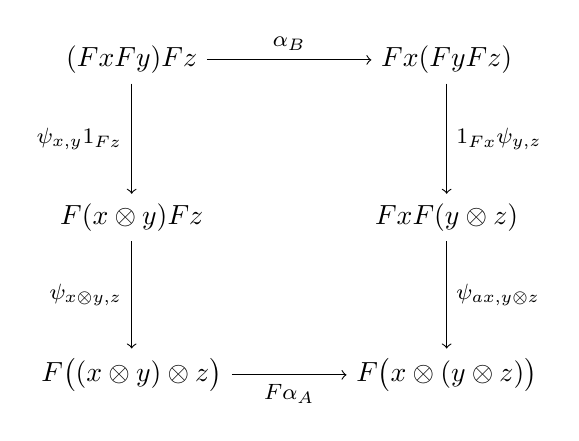
\begin{tikzpicture}
            \node (1) at (0, 0) {$(Fx\circledast Fy)\circledast Fz$};
            \node (2) at (4, 0) {$Fx\circledast(Fy\circledast Fz)$};
            \node (3) at (0, -2) {$F(x\otimes y)\circledast Fz$};
            \node (4) at (4, -2) {$Fx\circledast F(y\otimes z)$};
            \node (5) at (0, -4) {$F\bigl((x\otimes y)\otimes z\bigr)$};
            \node (6) at (4, -4) {$F\bigl(x\otimes(y\otimes z)\bigr)$};
            \draw[->] (1) -- node[above]{\footnotesize$\alpha_{\symbfsf{B}}$} (2);
            \draw[->] (5) -- node[below]{\footnotesize$F\alpha_{\symbfsf{A}}$} (6);
            \draw[->] (1) -- node[left]{\footnotesize$\psi_{x,y}\circledast\mathbbm{1}_{Fz}$} (3);
            \draw[->] (3) -- node[left]{\footnotesize$\psi_{x\otimes y,z}$} (5);
            \draw[->] (2) -- node[right]{\footnotesize$\mathbbm{1}_{Fx}\circledast\psi_{y,z}$} (4);
            \draw[->] (4) -- node[right]{\footnotesize$\psi_{ax,y\otimes z}$} (6);
        \end{tikzpicture}
        \caption{Monoidal functor.}
        \label{fig:monoidal_functor1}
    \end{figure}

    \newdef{Monoidal functor}{\index{monoidal!functor}\index{coherence!maps}
        Let $(\symbfsf{A},\otimes,\symbf{1}_{\symbfsf{A}}),(\symbfsf{B},\circledast,\symbf{1}_{\symbfsf{B}})$ be two monoidal categories. A functor $\func{F}{A}{B}$ is said to be monoidal if there exists:
        \begin{enumerate}
            \item a natural isomorphism $\psi_{x,y}:Fx\circledast Fy\Rightarrow F(x\otimes y)$ that makes the diagram in \cref{fig:monoidal_functor1} commute, and
            \item an isomorphism $\phi:\symbf{1}_{\symbfsf{B}}\rightarrow F\symbf{1}_{\symbfsf{A}}$ that makes the two diagrams in \cref{fig:unitality} commute.
        \end{enumerate}
        The maps $\psi$ and $\phi$ are also called \textbf{coherence maps} or \textbf{structure morphisms}.
    }

    \begin{figure}[ht!]
        \centering
        \begin{subfigure}[b]{0.49\textwidth}
            \centering
            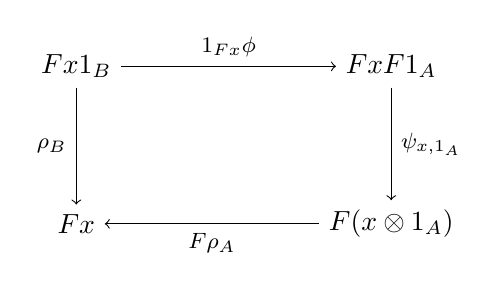
\begin{tikzpicture}
                \node (1) at (0, 0) {$Fx\circledast\symbf{1}_{\symbfsf{B}}$};
                \node (2) at (4, 0) {$Fx\circledast F\symbf{1}_{\symbfsf{A}}$};
                \node (3) at (0, -2) {$Fx$};
                \node (4) at (4, -2) {$F(x\otimes\symbf{1}_{\symbfsf{A}})$};
                \draw[->] (1) -- node[above]{\footnotesize$\mathbbm{1}_{Fx}\circledast\phi$} (2);
                \draw[<-] (3) -- node[below]{\footnotesize$F\rho_{\symbfsf{A}}$} (4);
                \draw[->] (1) -- node[left]{\footnotesize$\rho_{\symbfsf{B}}$} (3);
                \draw[->] (2) -- node[right]{\footnotesize$\psi_{x,\symbf{1}_{\symbfsf{A}}}$} (4);
            \end{tikzpicture}
        \end{subfigure}
        \begin{subfigure}[b]{0.49\textwidth}
            \centering
            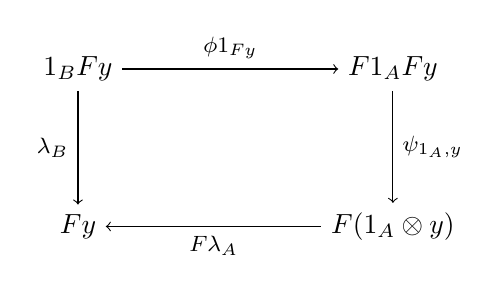
\begin{tikzpicture}
                \node (1) at (0, 0) {$\symbf{1}_{\symbfsf{B}}\circledast Fy$};
                \node (2) at (4, 0) {$F\symbf{1}_{\symbfsf{A}}\circledast Fy$};
                \node (3) at (0, -2) {$Fy$};
                \node (4) at (4, -2) {$F(\symbf{1}_{\symbfsf{A}}\otimes y)$};
                \draw[->] (1) -- node[above]{\footnotesize$\phi\circledast\mathbbm{1}_{Fy}$} (2);
                \draw[<-] (3) -- node[below]{\footnotesize$F\lambda_{\symbfsf{A}}$} (4);
                \draw[->] (1) -- node[left]{\footnotesize$\lambda_{\symbfsf{B}}$} (3);
                \draw[->] (2) -- node[right]{\footnotesize$\psi_{\symbf{1}_{\symbfsf{A}},y}$} (4);
            \end{tikzpicture}
        \end{subfigure}
        \caption{Unitality diagrams.}
        \label{fig:unitality}
    \end{figure}

    \begin{property}[Canonical unit]
        For every monoidal functor $F$, there exists a canonical isomorphism $\phi:\symbf{1}_{\symbfsf{B}}\rightarrow F\symbf{1}_{\symbfsf{A}}$ defined by the commutative diagram in \cref{fig:canonical_monoidal_isom}.

        \begin{figure}[ht!]
            \centering
            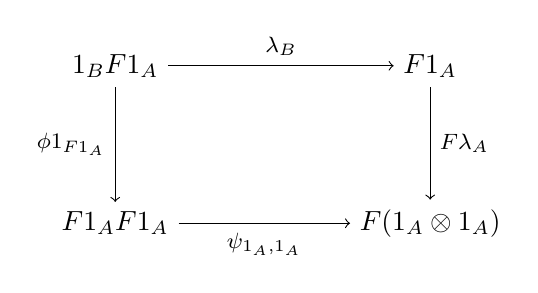
\begin{tikzpicture}
                \node (1) at (0, 0) {$\symbf{1}_{\symbfsf{B}}\circledast F\symbf{1}_{\symbfsf{A}}$};
                \node (2) at (4, 0) {$F\symbf{1}_{\symbfsf{A}}$};
                \node (3) at (0, -2) {$F\symbf{1}_{\symbfsf{A}}\circledast F\symbf{1}_{\symbfsf{A}}$};
                \node (4) at (4, -2) {$F(\symbf{1}_{\symbfsf{A}}\otimes\symbf{1}_{\symbfsf{A}})$};
                \draw[->] (1) -- node[above]{\footnotesize$\lambda_{\symbfsf{B}}$} (2);
                \draw[->] (3) -- node[below]{\footnotesize$\psi_{\symbf{1}_{\symbfsf{A}}, \symbf{1}_{\symbfsf{A}}}$} (4);
                \draw[->] (1) -- node[left]{\footnotesize$\phi\circledast\mathbbm{1}_{F\symbf{1}_{\symbfsf{A}}}$} (3);
                \draw[->] (2) -- node[right]{\footnotesize$F\lambda_{\symbfsf{A}}$} (4);
            \end{tikzpicture}
            \caption{Canonical unit isomorphism.}
            \label{fig:canonical_monoidal_isom}
        \end{figure}
    \end{property}

    \newdef{Lax monoidal functor}{\index{lax!monoidal functor}
        A monoidal functor for which the coherence maps are merely morphisms and not isomorphisms.
    }

    \newdef{Monoidal natural transformation}{
        A natural transformation $\eta$ between (lax) monoidal functors $(F,\psi,\phi_F)$ and $(G,\widetilde{\psi},\phi_G)$ that makes the diagrams in \cref{fig:monoidal_natural_transformation} commute.
        \begin{figure}[ht!]
            \centering
            \begin{subfigure}[b]{0.49\textwidth}
                \centering
                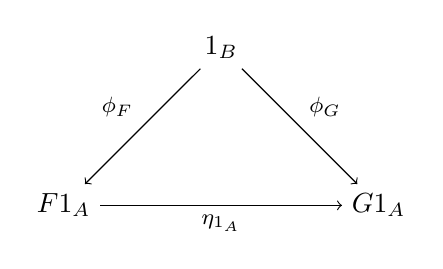
\begin{tikzpicture}
                    \node (1) at (0, 0) {$\symbf{1}_{\symbfsf{B}}$};
                    \node (2) at (-2, -2) {$F\symbf{1}_{\symbfsf{A}}$};
                    \node (3) at (2, -2) {$G\symbf{1}_{\symbfsf{A}}$};
                    \draw[->] (1) -- node[above left]{\footnotesize$\phi_F$} (2);
                    \draw[->] (1) -- node[above right]{\footnotesize$\phi_G$} (3);
                    \draw[->] (2) -- node[below]{\footnotesize$\eta_{\symbf{1}_{\symbfsf{A}}}$} (3);
                \end{tikzpicture}
            \end{subfigure}
            \begin{subfigure}[b]{0.49\textwidth}
                \centering
                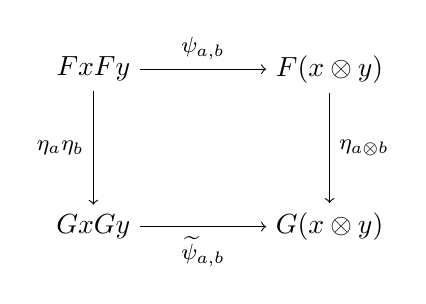
\begin{tikzpicture}
                    \node (1) at (0, 0) {$Fx\circledast Fy$};
                    \node (2) at (3, 0) {$F(x\otimes y)$};
                    \node (3) at (0, -2) {$Gx\circledast Gy$};
                    \node (4) at (3, -2) {$G(x\otimes y)$};
                    \draw[->] (1) -- node[above]{\footnotesize$\psi_{a,b}$} (2);
                    \draw[->] (3) -- node[below]{\footnotesize$\widetilde{\psi}_{a,b}$} (4);
                    \draw[->] (1) -- node[left]{\footnotesize$\eta_a\circledast\eta_b$} (3);
                    \draw[->] (2) -- node[right]{\footnotesize$\eta_{a\otimes b}$} (4);
                \end{tikzpicture}
            \end{subfigure}
            \caption{Monoidal natural transformation.}
            \label{fig:monoidal_natural_transformation}
        \end{figure}
    }

    \newdef{Monoidal equivalence}{\index{monoidal!equivalence}
        An equivalence of monoidal categories consisting of monoidal functors and monoidal natural isomorphisms.
    }
    \begin{theorem}[MacLane's strictness theorem]\index{MacLane!strictness theorem}
        Every monoidal category is monoidally equivalent to a strict monoidal category.
    \end{theorem}

\subsection{Closed categories}

    \newdef{Internal hom}{\index{internal!hom}\index{currying}\label{cat:internal_hom}
        Let $(\symbfsf{M},\otimes,\symbf{1})$ be a monoidal category. In this setting, one can generalize the \textit{currying} procedure, i.e.~the identification of maps $x\times y\rightarrow z$ with maps $x\rightarrow(y\rightarrow z)$. The internal hom-functor $\underline{\hom}$ is defined by the following natural isomorphism:
        \begin{gather}
            \symbfsf{M}(x\otimes y,z)\cong\symbfsf{M}\bigl(x,\underline{\hom}(y,z)\bigr).
        \end{gather}
        The existence of all internal homs is equivalent to the existence of a right adjoint to the tensor functor.
    }
    \begin{notation}
        The internal hom $\underline{\hom}(x,y)$ is also often denoted by $[x,y]$ (or $x\multimap y$). From now on, this convention will be followed (unless otherwise specified).
    \end{notation}
    \newdef{Closed monoidal category}{\index{closed!category}\index{Cartesian!closed}\label{cat:closed}
        A monoidal category that admits all internal homs. If the monoidal structure is induced by a (Cartesian) product structure, the category is often said to be \textbf{Cartesian closed}. A category for which all slice categories are Cartesian closed is said to be \textbf{locally Cartesian closed}.
    }
    \begin{property}
        A locally Cartesian closed category with a terminal object is Cartesian closed. Moreover, it is finitely complete. More generally, a locally Cartesian closed category has all pullbacks.
    \end{property}

    \newdef{Exponential object}{\index{exponential!object}\label{cat:exponential_object}
        In the case of Cartesian (monoidal) categories, the internal hom $[x,y]$ is called the exponential object. This object is often denoted by $y^x$.

        In Cartesian closed categories, a different, but frequently used, notation is $x\Rightarrow y$. However, this notation will not be used as it might be confused with the notation for \textit{2-morphisms}.
    }

    \newdef{Cartesian closed functor}{\index{Cartesian!closed}\label{cat:cartesian_closed_functor}
        A functor between Cartesian closed categories that preserves products and exponential objects. As such, it is the natural notion of functor between Cartesian closed categories.
    }
    \begin{property}[Frobenius reciprocity]\index{Frobenius!reciprocity}
        A functor $R$ between Cartesian closed categories that admits a left adjoint $L$ is Cartesian closed if and only if the natural transformation
        \begin{gather}
            L(y\times Rx)\rightarrow Ly\times x
        \end{gather}
        is a natural isomorphism.
    \end{property}

    \begin{property}[Global elements]\label{cat:internal_hom_property}
        The following isomorphism is natural in both $x,y\in\ob{M}$:
        \begin{gather}
            \symbfsf{M}\bigl(\symbf{1},[x,y]\bigr)\cong\symbfsf{M}(x,y)\,.
        \end{gather}
        It is this relation that gives the best explanation for the term `internal hom'. One also immediately obtains the following natural isomorphism:
        \begin{gather}
            \symbfsf{M}\bigl(x,[\symbf{1},y]\bigr)\cong\symbfsf{M}(x,y)\,.
        \end{gather}
        Because the Yoneda embedding is fully faithful, this implies that $[\symbf{1},y]\cong y$. Although the global elements $\symbfsf{M}(\symbf{1},y)$ do not fully specify an object $y$, this does hold internally.
    \end{property}

    \begin{property}[Symmetry]\label{cat:internal_symmetry}
        Let $\symbfsf{M}$ be a closed monoidal category. The definition of an internal hom can also be internalized, i.e.~there exists a natural isomorphism of the form
        \begin{gather}
            [x\otimes y,z]\cong[x,[y,z]]\,.
        \end{gather}
        Furthermore, if $\symbfsf{M}$ is also symmetric, there exists an internal isomorphism of the form
        \begin{gather}
            [x,[y,z]]\cong[y,[x,z]]\,.
        \end{gather}
    \end{property}

    \newdef{Strong adjunction}{\index{adjunction!strong}
        Consider a monoidal category $\symbfsf{M}$ together with two endofunctors $\func{L,R}{M}{M}$. These functors are said to form a strong adjunction if there exists a natural isomorphism
        \begin{gather}
            [Lx,y]\cong[x,Ry]\,.
        \end{gather}
        \Cref{cat:internal_hom_property} above implies that every strong adjunction is, in particular, an ordinary adjunction in the sense of \cref{section:adjunction}.
    }

\section{Enriched category theory}\label{section:enriched_category_theory}

    The following definition is due to \textit{B\'enabou}. It should represent the `ideal place in which to do category theory'.
    \newdef{Cosmos}{\index{cosmos}\label{cat:cosmos}
        A complete and cocomplete, closed symmetric monoidal category.
    }

    \newdef{Enriched category}{\index{category!enriched}
        Let $(\mathcal{V},\otimes,\symbf{1})$ be a monoidal category. A $\mathcal{V}$-enriched category, also called a $\mathcal{V}$-category\footnote{Not to be confused with the notation for fibre categories (\cref{cat:fibre_category}).}, consists of the following elements:
        \begin{itemize}
            \item a collection of objects $\ob{C}$, and
            \item for every pair of objects $x,y\in\ob{C}$, an object $\symbfsf{C}(x,y)\in\ob{\mathcal{V}}$ for which the following morphisms exist:
            \begin{enumerate}
                \item $\mathrm{id}_x:\symbf{1}\rightarrow\symbfsf{C}(x,x)$ giving the (enriched) identity morphism, and
                \item $\circ_{xyz}:\symbfsf{C}(y,z)\otimes\symbfsf{C}(x,y)\rightarrow\symbfsf{C}(x,z)$ replacing the usual composition.
            \end{enumerate}
        \end{itemize}
        The associativity and unity properties are given by commutative diagrams for the $\mathrm{id}$ and $\circ$ morphisms together with the associators and unitors in $\mathcal{V}$.
    }

    \newdef{Change of base}{\index{change of base}\label{cat:change_of_base}
        Consider a monoidal functor $\func{F}{\mathcal{V}}{\mathcal{W}}$. This induces a change-of-base functor $F_*:\mathcal{V}\symbfsf{Cat}\rightarrow\mathcal{W}\symbfsf{Cat}$ by applying $F$ to every hom-object.
    }

    \newdef{Underlying category}{
        Given a $\mathcal{V}$-enriched category $\symbfsf{C}$, the underlying category $\symbfsf{C}_0$ is defined as follows:
        \begin{itemize}
            \item\textbf{Objects}: $\ob{C}$, and
            \item\textbf{Morphisms}: $\mathcal{V}\bigl(\symbf{1},\symbfsf{C}(x,y)\bigr)$,
        \end{itemize}
        where $\symbf{1}$ is the monoidal unit in $\mathcal{V}$. This construction can be obtained as the functor $\mathcal{V}\symbfsf{Cat}(\mathcal{I},-)$, where $\mathcal{I}$ is the one-object $\mathcal{V}$-category with $\mathcal{I}(\ast,\ast):=\symbf{1}$.
    }
    \begin{property}[$\mathcal{V}$ as a $\mathcal{V}$-category]
        Consider a closed monoidal category $\mathcal{V}$. This category can be given the structure $\widetilde{\mathcal{V}}$ of a $\mathcal{V}$-category by taking the hom-objects to be the internal homs, i.e.~$\widetilde{\mathcal{V}}(x,y) := [x,y]$ for all $x,y\in\mathcal{V}$. \Cref{cat:internal_hom_property} then implies that there exists an isomorphism between the underlying category $\widetilde{\mathcal{V}}_0$ and the original category $\mathcal{V}$.
    \end{property}

    Given two $\mathcal{V}$-enriched categories, one can define suitable functors between them.
    \newdef{Enriched functor}{\index{functor}
        A $\mathcal{V}$-enriched functor $\func{F}{A}{B}$ consists of the following data:
        \begin{itemize}
            \item a function $F_0:\ob{A}\rightarrow\ob{B}$ (as for ordinary functors), and
            \item for every two objects $x,y\in\ob{A}$, a morphism $F_{x,y}:\symbfsf{A}(x,y)\rightarrow\symbfsf{B}(Fx,Fy)$ in $\mathcal{V}$.
        \end{itemize}
        These have to satisfy the `usual' composition and unit conditions.

        By extending \cref{cat:natural_end} using enriched ends, one obtains a definition of enriched natural transformations and, therefore, also a definition of enriched functor categories:
        \begin{gather}
            \label{cat:enriched_nat_end}
            \funccat{A}{B}(F,G) := \int_{x\in\symbfsf{A}}\symbfsf{B}(Fx,Gx)\,.
        \end{gather}
    }
    Given two $\mathcal{V}$-enriched functors $\func{F,G}{A}{B}$, one can also try to define $\mathcal{V}$-natural transformations by extending the usual definition of natural transformations (\cref{cat:natural}).
    \newdef{Enriched natural transformation}{\index{natural!transformation}
         An ordinary natural transformation consists of an $\ob{A}$-indexed family of morphism $\eta_x:Fx\rightarrow Gx$. This can also be interpreted as an $\ob{A}$-indexed family of morphisms $\eta_x:1\rightarrow\symbfsf{B}(Fx,Gx)$ from the initial object (one-element set). By analogy, a $\mathcal{V}$-natural transformation is defined as an $\ob{A}$-indexed family of morphisms $\eta_x:\symbf{1}\rightarrow\symbfsf{B}(Fx,Gx)$ from the monoidal unit. The usual naturality square is replaced by the naturality hexagon in \cref{fig:v_naturality}.
    }

    The question then becomes how these two definitions are related. The end in \cref{cat:enriched_nat_end} comes equipped with a projection $\varepsilon_x:\funccat{A}{B}(F,G)\rightarrow\symbfsf{B}(Fx,Gx)$. Precomposing this morphism with a morphism in the underlying category $\funccat{A}{B}_0$ exactly gives a $\mathcal{V}$-natural transformation. So, the underlying category of $\funccat{A}{B}$ is the ordinary category of $\mathcal{V}$-functors and $\mathcal{V}$-natural transformations.

     \begin{figure}
        \centering
        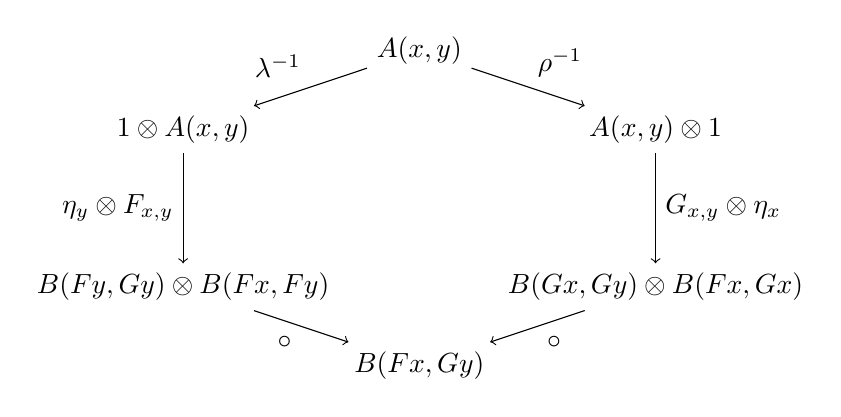
\begin{tikzpicture}
            \node (A) at (0, 0) {$\symbfsf{A}(x,y)$};
            \node (IA) at (-3, -1) {$\symbf{1}\otimes\symbfsf{A}(x,y)$};
            \node (AI) at (3, -1) {$\symbfsf{A}(x,y)\otimes\symbf{1}$};
            \node (BF) at (-3, -3) {$\symbfsf{B}(Fy,Gy)\otimes\symbfsf{B}(Fx,Fy)$};
            \node (BG) at (3, -3) {$\symbfsf{B}(Gx,Gy)\otimes\symbfsf{B}(Fx,Gx)$};
            \node (B) at (0, -4) {$\symbfsf{B}(Fx,Gy)$};
            \draw[->] (A) -- node[above left]{$\lambda^{-1}$} (IA);
            \draw[->] (A) -- node[above right]{$\rho^{-1}$} (AI);
            \draw[->] (IA) -- node[left]{$\eta_y\otimes F_{x,y}$} (BF);
            \draw[->] (AI) -- node[right]{$G_{x,y}\otimes\eta_x$} (BG);
            \draw[->] (BF) -- node[below left]{$\circ$} (B);
            \draw[->] (BG) -- node[below right]{$\circ$} (B);
        \end{tikzpicture}
        \caption{$\mathcal{V}$-naturality diagram.}
        \label{fig:v_naturality}
     \end{figure}

\subsection{Enriched constructions}

    \newdef{Functor tensor product}{\index{tensor product!of functors}\label{cat:functor_tensor_product}
        Consider a covariant functor $\func{G}{C}{\mathcal{V}}$ and a contravariant functor $\cfunc{F}{C}{\mathcal{V}}$ into a monoidal category $\mathcal{V}$, where $\symbfsf{C}$ does not have to be enriched over $\mathcal{V}$. The tensor product of $F$ and $G$ is defined as the following coend:
        \begin{gather}
            F\otimes_{\symbfsf{C}}G := \int^{x\in\symbfsf{C}}Fx\otimes Gx\,.
        \end{gather}
    }
    It should be noted that the above tensor product does not produce a new functor, instead it only gives an object in $\mathcal{V}$. A different type of tensor product, one that does give a functor, exists in the enriched setting (note that there is no relation between these two definitions).
    \newdef{Day convolution}{\index{Day convolution}
        Consider a monoidally cocomplete category $\mathcal{V}$, i.e.~cocomplete monoidal category for which the tensor product bifunctor is cocontinuous in each argument, together with a $\mathcal{V}$-enriched category $\symbfsf{C}$. The convolution or tensor product (if it exists) of two $\mathcal{V}$-enriched functors $\func{F,G}{C}{\mathcal{V}}$ is defined as the following coend:
        \begin{gather}
            F\otimes_{\mathrm{Day}}G := \iint^{x,y\in\symbfsf{C}}\symbfsf{C}(x\otimes y,-)\otimes Fx\otimes Gy\,.
        \end{gather}
    }
    \begin{property}[Monoidal structure]
        When $\symbfsf{M}$ is closed symmetric monoidal, Day convolution is associative and, hence, defines a monoidal structure on the functor category $\funccat{C}{M}$. The tensor unit is given by the functor (co)represented by the tensor unit in $\symbfsf{C}$.
    \end{property}

    \newdef{Copower}{\index{co-!power}\index{power}\label{hda:power} % Both terms are indexed since copowers are rather important on their own.
        Consider a $\mathcal{V}$-enriched category $\symbfsf{C}$. The copower (or \textbf{tensor}) functor $\func{\cdot}{\mathcal{V}\times C}{C}$ is defined by the following natural isomorphism:
        \begin{gather}
            \symbfsf{C}(v\cdot x,y)\cong\mathcal{V}\bigl(v,\symbfsf{C}(x,y)\bigr)\,.
        \end{gather}
        Dually, the \textbf{power} (or \textbf{cotensor}) functor $\func{[-,-]}{\mathcal{V}\times C}{C}$ is defined by the following natural isomorphism:
        \begin{gather}
            \symbfsf{C}\bigl(x,[v,y]\bigr)\cong\mathcal{V}\bigl(v,\symbfsf{C}(x,y)\bigr)\,.
        \end{gather}
        If an enriched category admits all (co)powers, it is said to be \textbf{(co)powered} (over its enriching category).
    }
    \remark{\Cref{cat:internal_symmetry} says that every (closed) symmetric monoidal category $\symbfsf{M}$ is powered over itself, the power just being the internal hom. The same holds for the copower, which is just the usual tensor product functor.}

    \begin{example}[Disjoint unions]
        Every (co)complete (locally) small category $\symbfsf{C}$ admits the structure of a $\symbfsf{Set}$-(co)powered category:
        \begin{gather}
            \begin{aligned}
                x^S &:= \prod_{s\in S}x\,,\\
                S\cdot x &:= \bigsqcup_{s\in S}x\,.
            \end{aligned}
        \end{gather}
    \end{example}

    The definition and properties of internal hom-functors and (co)powers can be formalized as follows.
    \newdef{Two-variable adjunction}{\index{adjunction}\label{cat:two_variable_adjunction}
        Consider three categories $\symbfsf{A,B}$ and $\symbfsf{C}$. A two-variable adjunction $\symbfsf{A}\times\symbfsf{B}\rightarrow\symbfsf{C}$ consists of three bifunctors:
        \begin{itemize}
            \item $\func{-\otimes-}{A\times B}{C}$,
            \item $\hom_L:\symbfsf{A}^{\text{op}}\times\symbfsf{C}\rightarrow\symbfsf{B}$, and
            \item $\hom_R:\symbfsf{B}^{\text{op}}\times\symbfsf{C}\rightarrow\symbfsf{A}$
        \end{itemize}
        admitting the following natural isomorphisms:
        \begin{gather}
            \symbfsf{C}(x\otimes y,z)\cong\symbfsf{A}\bigl(x,\hom_R(y,z)\bigr)\cong\symbfsf{B}\bigl(y,\hom_L(x,z)\bigr)\,.
        \end{gather}
        It should be noted that fixing any of the variables gives rise to ordinary adjunctions in the sense of \cref{section:adjunction}.
    }
    \begin{property}[Powers and copowers]
        A category $\symbfsf{C}$ enriched over a monoidal category $\mathcal{V}$ is powered and copowered over $\mathcal{V}$ exactly if the hom-functor $\symbfsf{C}^{\text{op}}\times\symbfsf{C}\rightarrow\mathcal{V}$ is the right adjoint in an enriched two-variable adjunction. The power and copower functors are then given by the other two adjoints.
    \end{property}

    The co-Yoneda lemma~\ref{cat:ninja_yoneda} can be generalized to the enriched setting.
    \begin{property}[Ninja Yoneda lemma]\index{Yoneda!reduction}\index{co-!Yoneda|see{Yoneda, reduction}}\label{cat:enriched_ninja_yoneda}
        Let $\cfunc{F}{C}{\mathcal{V}}$ be a contravariant functor (similar statements hold for covariant functors).
        \begin{gather}
            \begin{aligned}
                \int^{x\in\symbfsf{C}}\symbfsf{C}(-,x)\otimes Fx &\cong F\\
                \int_{x\in\symbfsf{C}}\mathcal{V}\bigl(\symbfsf{C}(x,-),Fx\bigr) &\cong F\,.
            \end{aligned}
        \end{gather}
    \end{property}

    The following definition constructs Kan extensions in the enriched setting (these can be shown to reduce to \cref{cat:kan_extension} when enriching over $\symbfsf{Set}$).
    \newadef{Kan extension}{\index{Kan!extension}\label{cat:enriched_kan_extension}
        Let $\symbfsf{A,B}$ and $\symbfsf{C}$ be categories enriched over a monoidal category $\mathcal{V}$. If $\symbfsf{B}$ is assumed to be copowered over $\mathcal{V}$, left Kan extension of $\func{F}{A}{B}$ along $\func{G}{A}{C}$ can be defined through a coend:
        \begin{gather}
            \mathrm{Lan}_GF := \int^{x\in\symbfsf{A}}\symbfsf{C}(Gx,-)\cdot Fx\,.
        \end{gather}
        If $\symbfsf{B}$ is assumed to be powered over $\mathcal{V}$, right Kan extension can be defined through an end:
        \begin{gather}
            \mathrm{Ran}_GF := \int_{x\in\symbfsf{A}}\bigl[\symbfsf{C}(-,Gx),Fx\bigr]\,.
        \end{gather}
        If $F$ is contravariant, the arguments of the hom-functors should simply be interchanged.
    }
    \remark{By choosing $\mathcal{V}=\symbfsf{Set},\symbfsf{C}=\symbfsf{A}$ and $G=\mathbbm{1}_{\symbfsf{A}}$ in the previous definition, one obtains the ninja Yoneda lemma~\ref{cat:ninja_yoneda}.}
    \begin{property}
        As already remarked in \cref{cat:preservation_kan_extension}, Kan extensions computed using (co)ends as above are strong.
    \end{property}

    \newadef{Functor tensor product}{\index{tensor product!of functors}\label{cat:copower_product}
        Let $\symbfsf{B}$ be a $\mathcal{V}$-enriched category. Consider a covariant functor $\func{G}{A}{B}$ and a contravariant functor $\cfunc{F}{A}{\mathcal{V}}$. The tensor product (\cref{cat:functor_tensor_product}) can be generalized whenever $\symbfsf{B}$ is copowered over $\mathcal{V}$:
        \begin{gather}
            F\otimes_{\symbfsf{A}}G := \int^{x\in\symbfsf{A}}Fx\cdot Gx\,.
        \end{gather}
    }

\subsection{Weighted (co)limits}\index{limit!weighted}\label{section:weighted_limits}

    In this section, the definition of ordinary limits and, in particular, the defining universal property~\ref{cat:limit_uproperty} is revisited. In this construction, the constant functor $\Delta_x$ was one of the main ingredients. This functor can be factorized as $\symbfsf{I}\rightarrow1\rightarrow\symbfsf{C}$, where $1$ denotes the terminal category. At the level of morphisms, this factorization takes the form $\symbfsf{I}(i,j)\rightarrow\ast\rightarrow\symbfsf{C}(x,x)$, where $\ast$ denotes the terminal one-element set. However, whenever the enriching context is not $\symbfsf{Set}$, one does not necessarily have access to a terminal object.

    To avoid this issue, limits will first be redefined as representing objects. To this end, consider a general diagram $\func{D}{I}{C}$. By postcomposition with the Yoneda embedding, one obtains the presheaf-valued diagram $\symbfsf{C}(-,D-):\symbfsf{I}\rightarrow[\symbfsf{C}^{\text{op}},\symbfsf{Set}]$. Since presheaf categories are complete (\cref{cat:complete_presheaf_category}), the limit of this diagram exists:
    \begin{gather}
        \symbfsf{Set}\bigl(S,\lim\symbfsf{C}(x,D-)\bigr)\cong\funccat{I}{Set}\bigl(\Delta_S,\symbfsf{C}(x,D-)\bigr)\,.
    \end{gather}
    By restricting to the terminal set $S=\ast$, one obtains
    \begin{gather}
        \lim\symbfsf{C}(x,D-)\cong\funccat{I}{Set}\bigl(\Delta_\ast,\symbfsf{C}(x,D-)\bigr)\,.
    \end{gather}
    If this presheaf is representable, one can use the continuity of the hom-functor, together with the fact that the Yoneda embedding is fully faithful, to show that the representing object is (isomorphic to) $\lim D$, i.e.
    \begin{gather}
        \funccat{I}{Set}\bigl(\Delta_\ast,\symbfsf{C}(x,D-)\bigr)\cong\symbfsf{C}(x,\lim D)\,.
    \end{gather}

    \todo{CLEAN THIS UP (note that continuity and pointwise definition was already mentioned for ordinary limits)}

    \newdef{Weighted limit}{\index{limit!conical}\label{cat:weighted_limit}
        The above construction can now be generalized by replacing the constant functor $\Delta_\ast$ by any functor $\func{W}{I}{Set}$. A representing object is then called the $W$-weighted limit of $D$. This object is often denoted by $\wlim{W}D$ or $\{W,D\}$. To distinguish weighted limits from ordinary ones, the latter are sometimes called \textbf{conical limits}.
    }

    \begin{remark}
        A motivation for this construction is the following. As was already pointed out in \cref{cat:global_elements_remark}, the mere knowledge of global elements $1\rightarrow x$ is often not enough to characterize an object $x$. In general, one should look at the collection of generalized elements. When applying this ideology to the case of cones, one sees that replacing the functor $\Delta_\ast$ by a more general functor is the same as replacing the global elements $\ast\rightarrow Di$ by generalized elements $Wi\rightarrow Di$.
    \end{remark}

    The generalization to the enriched setting is now evident. There is no reference to the terminal object left, so one can replace $\symbfsf{Set}$ by any enriching category. In the enriched setting, (co)end formulas for (weighted) limits will often be used.
    \newformula{Enriched weighted limits}{\label{cat:weighted_limits}
        By expressing the natural transformations as an end as in \cref{cat:natural_end} and by using the canonical powering in $\symbfsf{Set}$, one can express ordinary weighted limits as follows:
        \begin{gather}
            \wlim{W}D\cong\int_{i\in\symbfsf{I}}[Wi,Di]\,.
        \end{gather}
        The generalization to other enriching categories is now straightforward. Consider a diagram $\func{D}{I}{C}$ and a weight functor $\func{W}{I}{\mathcal{V}}$, where $\symbfsf{C}$ is $\mathcal{V}$-enriched. If $\symbfsf{C}$ is powered over $\mathcal{V}$, the $W$-weighted limit of $D$ is defined by the same formula as above:
        \begin{gather}
            \wlim{W}D:=\int_{i\in\symbfsf{I}}[Wi,Di]\,.
        \end{gather}
        In a similar way, one can define weighted colimits in copowered $\mathcal{V}$-categories as coends:
        \begin{gather}
            \colim^WD:=\int^{i\in\symbfsf{I}}Wi\cdot Di\,.
        \end{gather}
        Here, the weight functor $W$ is required to be contravariant since colimits (and cocones in general) are natural transformations between contravariant functors.
    }
    \begin{property}[Weighted limits are Homs]
        In the case $\symbfsf{C}=\mathcal{V}$, the powering becomes the internal hom and, therefore, one sees that weighted limits are given by (enriched) natural transformations (as was the case for ordinary conical limits).
    \end{property}

    In the following example, the weighted colimit is calculated with respect to the Yoneda embedding.
    \begin{example}[Hom-functor]
        Consider a diagram $\func{D}{I}{C}$. When using the Yoneda embedding $\mathcal{Y}i = \symbfsf{I}(-,i)$ as the weight functor, one obtains the following property by virtue of the Yoneda lemma:
        \begin{gather}
            \label{cat:weighted_hom_colimit}
            \colim^{\mathcal{Y}i}D\cong Di\,.
        \end{gather}
        A similar statement for weighted limits can be obtained with the covariant Yoneda embedding.
    \end{example}
    \newadef{Weighted (co)limits}{\index{limit!weighted}
        The above property can be used to axiomatize small weighted (co)limits in bicomplete categories:
        \begin{enumerate}
            \item\textbf{Yoneda}: For every object $i\in\ob{I}$, there exist isomorphisms
            \begin{gather}
                \wlim{\symbfsf{I}(i,-)}D\cong Di\qquad\text{and}\qquad\colim^{\symbfsf{I}(-,i)}D\cong Di\,.
            \end{gather}
            \item\textbf{Cocontinuity}: The weighted (co)limit functors are cocontinuous in the weights.
        \end{enumerate}
    }

    One can also express Kan extensions as weighted limits (this simply follows from \cref{cat:enriched_kan_extension}).
    \begin{property}[Kan extensions]\index{Kan!extension}
        Consider functors $\func{F}{A}{B}$ and $\func{G}{A}{C}$. If, for every $x\in\ob{C}$, the weighted limit $\wlim{\symbfsf{C}(x,G-)}F$ exists, these limits can be combined into a functor that can be shown to be the right Kan extension $\mathrm{Ran}_GF$. The left Kan extension can be obtained as a weighted colimit.
    \end{property}

    \begin{property}[Category of elements]\index{category!of elements}
        The weighted (co)limits of a functor (over $\symbfsf{Set}$) can also be expressed in terms of the category of elements (\cref{cat:category_of_elements}) of the weight:
        \begin{gather}
            \wlim{W}F\cong\lim F\circ\symbfsf{C}_W\,,
        \end{gather}
        where the limit on the right-hand side is a conical limit.

        The reason for the (co)end notation for categories of elements can also be explained by noting that these can actually be obtained as weighted (co)limits or (co)ends (here given for covariants functors):
        \begin{gather}
            \mathrm{El}(F) \cong \int^{c\in\symbfsf{C}}Jc\times\mathrm{Disc}\,Fc\,,
        \end{gather}
        where $\cfunc{J}{C}{Cat}:c\mapsto c/\symbfsf{C}$ assigns undercategories and $\func{\mathrm{Disc}}{Set}{Cat}$ sends sets to discrete categories.
    \end{property}

\section{Abelian categories}\label{section:abelian_categories}
\subsection{Additive categories}

    \newdef{Pre-additive category}{
        A (locally small) category enriched over $\symbfsf{Ab}$, i.e.~a category in which every hom-set is an Abelian group and composition is bilinear.
    }

    \begin{property}\index{zero!object}
        Let $\symbfsf{A}$ be a pre-additive category. The following statements are equivalent for an object $x\in\ob{A}$:
        \begin{itemize}
            \item $x$ is initial,
            \item $x$ is final, or
            \item $\mathbbm{1}_x = 0$.
        \end{itemize}
        It follows that every initial/terminal object in a pre-additive category is automatically a zero object (\cref{cat:zero_object}).
    \end{property}
    \begin{property}[Biproducts]\index{bi-!product}\index{direct!sum}
        In a pre-additive category, the following isomorphism holds for all finitely indexed sets $\{x_i\}_{i\leq n}$:
        \begin{gather}
            \prod_{i\leq n}x_i\cong\bigsqcup_{i\leq n}x_i\,.
        \end{gather}
        Finite (co)products in pre-additive categories are often called \textbf{direct sums}. In general, if a product and coproduct exist and are isomorphic, one also speaks of a \textbf{biproduct}.
    \end{property}

    \newdef{Additive category}{\index{additive!category}
        A pre-additive category admitting all finite products (and, hence, biproducts).
    }

    When working with additive categories, it is generally assumed that the associated functors are of a specific type.
    \newdef{Additive functor}{\index{additive!functor}\label{cat:additive_functor}
        Let $\symbfsf{A},\symbfsf{A'}$ be additive categories. A functor $\func{F}{A}{A'}$ is said to be additive if it preserves finite biproducts:
        \begin{enumerate}
            \item It preserves zero objects: $F\,0_{\symbfsf{A}}\cong0_{\symbfsf{A}'}$.
            \item There exists a natural isomorphism $F(x\oplus y)\cong Fx\oplus Fy$.
        \end{enumerate}
        This notion can be generalized to pre-additive categories. A functor between pre-additive categories is said to be additive if it acts by group morphisms on hom-spaces.
    }

    \newdef{Grothendieck group}{\index{Grothendieck!group}
        Let $\symbfsf{A}$ be an additive category and consider its decategorification (\cref{cat:decategorification}). This set carries the structure of an Abelian monoid and, hence, the Grothendieck construction (\cref{group:grothendieck_completion}) can be applied to obtain an Abelian group $K(\symbfsf{A})$. This group is called the Grothendieck group of $\symbfsf{A}$.
    }

    In a (pre-)additive category, one can define some classical notions from (homological) algebra such as images and kernels.
    \newdef{Kernel}{\index{kernel}
        Let $f:x\rightarrow y$ be a morphism. A\footnote{`\textit{A}' since the kernel of a morphism is only determined up to an isomorphism.} kernel of $f$ is a morphism $k:z\rightarrow x$ such that:
        \begin{gather}
            f\circ k = 0
        \end{gather}
        and such that it is universal with respect to this property. This implies that a kernel of $f$ could equivalently be defined as the equalizer of $f$ and $0$.
    }
    \begin{notation}[Kernel]
        If the kernel of $f:x\rightarrow y$ exists, it is denoted by $\ker(f)$.
    \end{notation}

    \newdef{Cokernel}{
        Let $f:x\rightarrow y$ be a morphism. A cokernel of $f$ is a morphism $p:y\rightarrow z$ such that:
        \begin{gather}
            p\circ f = 0
        \end{gather}
        and such that it is universal with respect to this property. This implies that a cokernel of $f$ could equivalently be defined as the coequalizer of $f$ and 0.
    }
    \begin{notation}[Cokernel]
        If the cokernel of $f:x\rightarrow y$ exists, it is denoted by $\mathrm{coker}(f)$.
    \end{notation}

    \begin{remark}
        The name and notation of the kernel and the cokernel (in the categorical sense) are explained by remarking that $\ker(f)$ represents the functor
        \begin{gather}
            F:z\mapsto\ker\bigl(\symbfsf{C}(z,x)\rightarrow\symbfsf{C}(z,y)\bigr)\,,
        \end{gather}
        where $\ker$ denotes the algebraic kernel (\cref{group:kernel}), and similarly for the cokernel.
    \end{remark}

    \newdef{Pseudo-Abelian category}{\label{cat:pseudo_abelian}
        An additive category in which every projection/idempotent has a kernel.
    }
    \newdef{Pre-Abelian category}{
        An additive category in which every morphism has a kernel and cokernel.
    }
    \newdef{Abelian category}{\index{Abelian!category}
        A pre-Abelian category in which every mono is a kernel and every epi is a cokernel or, equivalently, if for every morphism $f$ there exists an isomorphism
        \begin{gather}
            \coker\bigl(\ker(f)\bigr)\cong\ker\bigl(\coker(f)\bigr)\,.
        \end{gather}
    }

    \begin{property}
        Every Abelian category is balanced (\cref{cat:balanced}).
    \end{property}

    \begin{property}[Injectivity and surjectivity]
        In Abelian categories, a morphism is monic if and only if it is injective, i.e.~its kernel is 0. Analogously, a morphism is epic if and only if it is surjective, i.e.~its cokernel is 0.
    \end{property}

    \newdef{Linear category}{\index{category!linear}
        Let $\symbfsf{Vect}_k$ denote the category of vector spaces over the base field $k$. A $k$-linear category is a category enriched over $\symbfsf{Vect}_k$. (If the base field is clear, it is often left implicit.)
    }

\subsection{Exact functors}

    In the setting of additive categories, \cref{cat:exact_functor} can be characterized more simply.
    \newdef{Exact functor}{\index{exact!functor}
        Let $\func{F}{A}{A'}$ be an additive functor between additive categories.
        \begin{itemize}
            \item $F$ is left exact if it preserves kernels.
            \item $F$ is right exact if it preserves cokernels.
            \item $F$ is exact if it is both left and right exact.
        \end{itemize}
    }
    \begin{result}
        The previous definition implies the following properties (which can, in fact, be used as an alternative definition):
        \begin{itemize}
            \item If $F$ is left exact, it maps an exact sequence of the form \[0\longrightarrow x\longrightarrow y\longrightarrow z\]
            to an exact sequence of the form \[0\longrightarrow Fx\longrightarrow Fy\longrightarrow Fz\,.\]
            \item If $F$ is right exact, it maps an exact sequence of the form \[x\longrightarrow y\longrightarrow z\longrightarrow 0\]
            to an exact sequence of the form \[Fx\longrightarrow Fy\longrightarrow Fz\longrightarrow 0\,.\]
            \item If $F$ is exact, it maps short exact sequences to short exact sequences.
        \end{itemize}
    \end{result}

    \begin{notation}[Left or right]
        The category of left modules ${}_R\symbfsf{Mod}$ over a ring $R$ is equivalent (as an Abelian category) to the category of right modules $\symbfsf{Mod}_{\op{R}}$ over the opposite ring $R$. For this reason, one often makes no difference between left and right modules (only bimodules are truly relevant) and `the category of $R$-modules' is just denoted by $R\symbfsf{Mod}$.
    \end{notation}

    \begin{theorem}[Freyd--Mitchell embedding theorem]\index{Freyd--Mitchell embedding theorem}\index{embedding!theorem|see{Freyd--Mitchell}}\label{cat:freyd_mitchell}
        Every small Abelian category admits a fully faithful, exact functor into a category of the form $R\symbfsf{Mod}$ for some unital ring $R$.
    \end{theorem}

    \begin{theorem}[Eilenberg--Watts]\index{Eilenberg--Watts}
        Let $R,S$ be two (not necessarily unital) rings. The tensor product functor induces an equivalence between the category of $R\text{-}S$-bimodules and the category of cocontinuous functors $R\symbfsf{Mod}\rightarrow S\symbfsf{Mod}$.
    \end{theorem}

\subsection{Finiteness}

    \newdef{Simple object}{\index{simple!object}
        Let $\symbfsf{A}$ be an Abelian category. An object $a\in\ob{A}$ is said to be simple if the only subobjects of $a$ are $0$ and $a$ itself. An object is said to be semisimple if it is a direct sum of simple obejcts.
    }
    \newdef{Semisimple category}{
        A category is said to be semisimple if every object is semisimple, where, in general, the direct sums are taken over finite index sets.
    }

    \newdef{Jordan--H\"older series}{\index{finite}\index{Jordan--H\"older!series}
        A filtration (\cref{set:filtration})
        \begin{gather}
            0\longrightarrow x_1\longrightarrow x_2\longrightarrow\cdots\longrightarrow x_n=x
        \end{gather}
        of an object $x$ is said to be a Jordan--H\"older series if the quotient objects $x_i/x_{i-1}$ are simple for all $i\leq n$. If the series has finite length, the object $x$ is said to be \textbf{finite}.
    }
    \begin{theorem}[Jordan--H\"older]\index{Jordan--H\"older}
        If an object in an Abelian category is finite, all of its Jordan--H\"older series have the same length. In particular, the multiplicities of simple objects are the same for all such series.
    \end{theorem}

    \begin{theorem}[Krull--Schmidt]\index{Krull--Schmidt}\index{indecomposable}
        Any object in an Abelian category of finite length admits a unique decomposition as a direct sum of indecomposable objects\footnote{An object is \textbf{indecomposable} if it cannot be written as a direct sum of its subobjects.}.
    \end{theorem}

    \newdef{Locally finite}{\label{cat:locally_finite}
        A $\mathfrak{K}$-linear Abelian category is said to be locally finite if it satisfies the following conditions:
        \begin{enumerate}
            \item every hom-space is finite-dimensional, and
            \item every object has finite length.
        \end{enumerate}
    }
    \newdef{Finite}{\index{finite}\index{projective!cover}
        A $\mathfrak{K}$-linear Abelian category is said to be finite if it satisfies the following conditions:
        \begin{enumerate}
            \item it is locally finite,
            \item it has enough projectives or, equivalently, every simple object has a \textit{projective cover}, and
            \item the set of isomorphism classes of simple objects is finite.
        \end{enumerate}
    }

    \begin{theorem}[Schur's lemma]\index{Schur!lemma}\label{cat:schur_lemma}
        Let $\symbfsf{A}$ be an Abelian category. For every two simple objects $x,y\in\ob{A}$, all nonzero morphisms $x\rightarrow y$ are isomorphisms. In particular, if $x,y$ are two non-isomorphic simple objects, then $\symbfsf{A}(x,y)=0$. Furthermore, $\symbfsf{A}(x,x)$ is a division ring for every simple object $x\in\ob{A}$.
    \end{theorem}
    \begin{result}
        If $\symbfsf{A}$ is locally finite and $\mathfrak{K}$ is algebraically closed, then $\symbfsf{A}(x,x)\cong\mathfrak{K}$ for all simple objects $x\in\ob{A}$. This follows from the fact that the only finite-dimensional division algebra over an algebraically closed field is the field itself.
    \end{result}

    The Freyd--Mitchell theorem~\ref{cat:freyd_mitchell} can be adapted to the finite linear case as follows.
    \begin{theorem}[Deligne]\index{Deligne}
        Every finite $\mathfrak{K}$-linear Abelian category is $\mathfrak{K}$-linearly equivalent to a category of the form $A\symbfsf{Mod}^{\emph{fin}}$ for $A$ a finite-dimensional $\mathfrak{K}$-algebra.
    \end{theorem}

    \begin{construct}[Deligne tensor product]\index{Deligne|seealso{tensor product}}\index{tensor product!Deligne}
        Let $\symbfsf{A},\symbfsf{B}$ be two Abelian categories. Their Deligne (tensor) product is defined (if it exists) as the category $\symbfsf{A}\boxtimes\symbfsf{B}$ for which there exists a bijection between right exact functors $\symbfsf{A}\boxtimes\symbfsf{B}\rightarrow\symbfsf{C}$ and right exact functors $\symbfsf{A}\times\symbfsf{B}\rightarrow\symbfsf{C}$ (the latter being right exact in each argument).

        For finite Abelian categories, it can be shown that their Deligne product always exists. By the Deligne embedding theorem, one can find an explicit description. Consider two finite-dimensional $\mathfrak{K}$-algebras $A,B$. The category $A\symbfsf{Mod}^{\text{fin}}\boxtimes B\symbfsf{Mod}^{\text{fin}}$ is equivalent to the category $(A\otimes_{\mathfrak{K}}B)\symbfsf{Mod}^{\text{fin}}$.
    \end{construct}

\section{Duality}\label{section:duality}

    \newdef{Dual object}{\index{dual!object}\index{evaluation}\index{unit}\label{hda:dual}
        Let $(\symbfsf{C},\otimes,\symbf{1})$ be a monoidal category and consider an object $x\in\ob{C}$. A left dual\footnote{$x$ is called the \textbf{right dual} of $x^*$. The right dual of $y$ is often denoted by ${}^*y$.} of $x$ is an object $x^*\in\ob{C}$ together with two morphisms $\eta:\symbf{1}\rightarrow x\otimes x^*$ and $\varepsilon:x^*\otimes x\rightarrow\symbf{1}$, called the \textbf{unit} and \textbf{counit} morphisms\footnote{Also called the \textbf{coevaluation} and \textbf{evaluation} morphisms.}, such that the diagrams in \cref{fig:dual_objects} commute. $x$ is said to be \textbf{dualizable} if it admits a left dual.
    }

    \begin{figure}[ht!]
        \centering
        \begin{subfigure}[b]{0.49\textwidth}
            \centering
            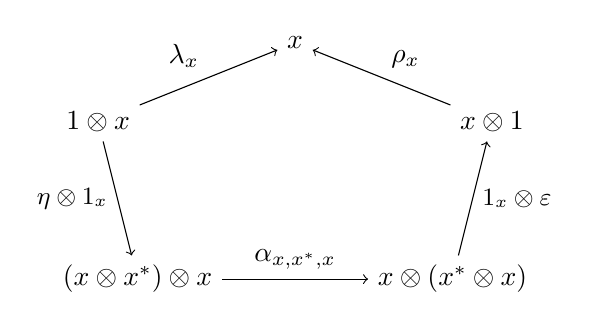
\begin{tikzpicture}
                \node (X) at (0, 0) {$x$};
                \node (1X) at (-2.5, -1) {$\symbf{1}\otimes x$};
                \node (X1) at (2.5, -1) {$x\otimes\symbf{1}$};
                \node (1XXX) at (-2, -3) {$(x\otimes x^*)\otimes x$};
                \node (XXX1) at (2, -3) {$x\otimes(x^*\otimes x)$};
                \draw[->] (1X) -- node[above left]{$\lambda_x$} (X);
                \draw[->] (X1) -- node[above right]{$\rho_x$} (X);
                \draw[->] (1X) -- node[left]{\small $\eta\otimes\mathbbm{1}_x$} (1XXX);
                \draw[->] (XXX1) -- node[right]{\small $\mathbbm{1}_x\otimes\varepsilon$} (X1);
                \draw[->] (1XXX) -- node[above]{$\alpha_{x,x^*,x}$} (XXX1);
            \end{tikzpicture}
            \caption{Dual object I.}
            \label{fig:dual_object1}
        \end{subfigure}
        \begin{subfigure}[b]{0.49\textwidth}
            \centering
            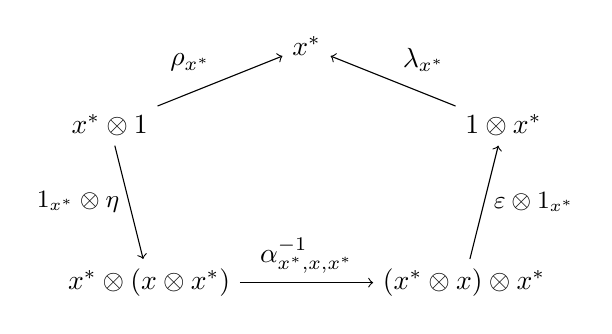
\begin{tikzpicture}
                \node (X) at (0, 0) {$x^*$};
                \node (X1) at (-2.5, -1) {$x^*\otimes\symbf{1}$};
                \node (1X) at (2.5, -1) {$\symbf{1}\otimes x^*$};
                \node (XXX1) at (-2, -3) {$x^*\otimes(x\otimes x^*)$};
                \node (1XXX) at (2, -3) {$(x^*\otimes x)\otimes x^*$};
                \draw[->] (X1) -- node[above left]{$\rho_{x^*}$} (X);
                \draw[->] (1X) -- node[above right]{$\lambda_{x^*}$} (X);
                \draw[->] (X1) -- node[left]{\small $\mathbbm{1}_{x^*}\otimes\eta$} (XXX1);
                \draw[->] (1XXX) -- node[right]{\small $\varepsilon\otimes\mathbbm{1}_{x^*}$} (1X);
                \draw[->] (XXX1) -- node[above]{$\alpha^{-1}_{x^*,x,x^*}$} (1XXX);
            \end{tikzpicture}
            \caption{Dual object II.}
            \label{fig:dual_object2}
        \end{subfigure}
        \caption{Dualizable objects.}
        \label{fig:dual_objects}
    \end{figure}

    \newdef{Rigid category}{\index{category!rigid}\index{category!autonomous}
        A monoidal category that has all duals. These categories are also said to be \textbf{autonomous}. If only left (resp.~right) duals exist, the category is said to be left (resp.~right) rigid.
    }

    \begin{property}[Braided categories]\label{hda:braided_rigid}
        In general, it is not true that left and right duals coincide. However, in a braided monoidal category this is the case.
    \end{property}

    \newdef{Compact closed category}{\index{category!compact closed}
        A symmetric rigid category.
    }

    \begin{example}[FinVect]\index{dual!space}\index{resolution!of the identity}
        Consider the category $\symbfsf{FinVect}$ of finite-dimensional vector spaces (the ground field is assumed to be $\mathbb{R}$). The categorical dual of a vector space $V$ is the algebraic dual $V^*$. The unit morphism is given by the `resolution of the identity':
        \begin{gather}
            \eta:\symbf{1}\rightarrow V\otimes V^*:1\mapsto\sum_{i=1}^{\dim(V)}e_i\otimes\phi^i\,,
        \end{gather}
        where $\{e_i\}$ and $\{\phi^i\}$ are dual bases of $V$ and $V^*$, respectively.

        It should be noted that the category $\symbfsf{Vect}$ of all vector spaces is not rigid. By \cref{hda:braided_rigid} above, left and right duals coincide in any braided monoidal category (such as $\symbfsf{Vect}$), but for infinite-dimensional vector spaces it is known that $A\cong(A^*)^*$ never holds and, as such, rigidity cannot be extended to $\symbfsf{Vect}$.
    \end{example}

    \begin{property}[Tannaka duality]\index{Tannaka duality}
        Consider the category $\mathcal{V}=\symbfsf{FinVect}_k$. Using coends, one can reconstruct the base field from its modules, i.e.~the objects in $\mathcal{V}$:
        \begin{gather}
            \int^{V\in\mathcal{V}}V^*\otimes V\cong k\,.
        \end{gather}
        This result can be shown to hold for all compact closed categories $\mathcal{V}$. In this context, it is known as \textbf{Tannaka reconstruction}. A more general statement goes as follows:
        \begin{gather}
            \int^{V\in\mathcal{V}}\mathcal{V}(V,-)\otimes V\cong\mathrm{id}_{\mathcal{V}}\,.
        \end{gather}
        For $\mathcal{V}=\symbfsf{FinVect}_k$, the components $\eta_V:\mathcal{V}(V,V)\rightarrow k$ of the coend can be shown to coincide with the trace and, as such, the trace obtains a universal property.
    \end{property}
    \begin{remark}
        This property can also be generalized by replacing $\mathcal{V}$ by a category of modules $A\symbfsf{Mod}$ for some finite-dimensional algebra $A$. The end and coend give the algebra $A$ and its dual $A^*$, respectively.
    \end{remark}

    For certain purposes, it is useful to slightly weaken the notion of compact closed categories (e.g.~\citet{kissinger_categorical_2019,barr_-autonomous_1991}).
    \newdef{$\ast$-autonomous category}{\index{category!autonomous}\label{hda:star_autonomous_category}
        A symmetric monoidal category $(\symbfsf{C},\otimes,\symbf{1})$ with a fully faithful dualization functor $\cfunc{\ast}{C}{C}$ such that
        \begin{gather}
            \symbfsf{C}(x\otimes y,z^*)\cong\symbfsf{C}\bigl(x,(y\otimes z)^*\bigr)
        \end{gather}
        for all $x,y,z\in\ob{C}$.
    }
    \begin{property}[de Morgan duality]\index{de Morgan!duality}\label{hda:de_morgan_duality}
        If $(\symbfsf{C},\otimes,\symbf{1},\ast)$ is a $\ast$-autonomous category, it admits a second $\ast$-autonomous structure $(\symbfsf{C},\dualampersand,\bot,\ast)$ given by
        \begin{gather}
            x\dualampersand y := (x^*\otimes y^*)^*
        \end{gather}
        for all $x,y\in\ob{C}$ and
        \begin{gather}
            \bot := \symbf{1}^*\,.
        \end{gather}
    \end{property}

    \begin{property}[Involution]
        Note that the definition of $\ast$-autonomous categories implies that
        \begin{gather}
            x\cong x^{**}
        \end{gather}
        for all $x\in\ob{C}$. Moreover, $\ast$-autonomous categories are closed with the internal hom given by:
        \begin{gather}
            [x,y] = x^*\dualampersand y \cong (x\otimes y^*)^*\,.
        \end{gather}
        A $\ast$-autonomous category is compact closed if and only if duality is compatible with tensor products:
        \begin{gather}
            (x\otimes y)^*\cong x^*\otimes y^*\,.
        \end{gather}
        Equivalently, a $\ast$-autonomous category is compact closed if and only if the de Morgan-dual monoidal structures coincide.
    \end{property}

    \newdef{Symmetric monoidal dagger category}{\index{category!dagger}
        A symmetric monoidal category $(\symbfsf{C},\otimes,\symbf{1})$ that also carries the structure of a dagger category (\cref{cat:dagger_category}) such that
        \begin{gather}
            (f\otimes g)^\dag = f^\dag\otimes g^\dag
        \end{gather}
        and such that the coherence and braiding morphisms are unitary.
    }
    \newdef{Dagger-compact category}{
        A symmetric monoidal dagger category that is also a compact closed category such that the following diagram commutes for all objects:
        \begin{gather*}
            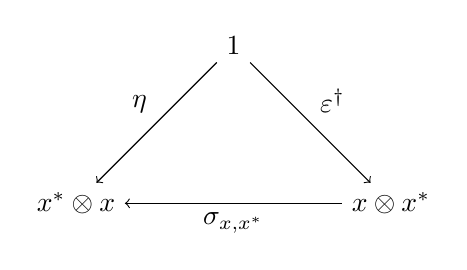
\begin{tikzpicture}
                \node (1) at (0, 0) {$\symbf{1}$};
                \node (X*X) at (-2, -2) {$x^*\otimes x$};
                \node (XX*) at (2, -2) {$x\otimes x^*$};
                \draw[->] (1) -- node[above left]{$\eta$} (X*X);
                \draw[->] (1) -- node[above right]{$\varepsilon^\dagger$} (XX*);
                \draw[<-] (X*X) -- node[below]{$\sigma_{x,x^*}$} (XX*);
            \end{tikzpicture}
        \end{gather*}
    }

    The trace on $\symbfsf{FinVect}$ can be generalized as follows.
    \newdef{Trace}{\index{trace}
        Let $(\symbfsf{C},\otimes,\symbf{1})$ be a rigid category and consider $f\in\symbfsf{C}(x,x^{**})$. The left (\textbf{categorical} or \textbf{quantum}) trace of $f$ is defined as the following morphism in $\End_{\symbfsf{C}}(\symbf{1})$:
        \begin{gather}
            \tr^L(f):=\varepsilon_{x^*}\circ(f\otimes\mathbbm{1}_{x^*})\circ\eta_x\,.
        \end{gather}
        For $f\in\symbfsf{C}(x,{}^{**}x)$, the right trace is defined similarly:
        \begin{gather}
            \tr^R(f):=\varepsilon_{{}^{**}x}\circ(\mathbbm{1}_x\otimes f)\circ\eta_{{}^*x}\,.
        \end{gather}
    }
    \begin{property}
        The following linear algebra-like properties hold for the categorical trace:
        \begin{itemize}
            \item $\tr^L(f) = \tr^R(f^*)$,
            \item $\tr^L(f\otimes g) = \tr^L(f)\tr^L(g)$, and
            \item for additive categories: $\tr^L(f\oplus g) = \tr^L(f) + \tr^L(g)$.
        \end{itemize}
        The second and third property can be stated analogously for the right trace.
    \end{property}

    \newdef{Pivotal category}{\index{pivotal structure}
        Let $\symbfsf{C}$ be a rigid monoidal category. A pivotal structure on $\symbfsf{C}$ is a monoidal natural isomorphism $\psi:\mathrm{id}_{\symbfsf{C}}\Rightarrow\ast\ast$.
    }

    \newdef{Dimension}{\index{dimension!pivotal}\label{hda:pivotal_dimension}
        Let $(\symbfsf{C},\psi)$ be a pivotal category and consider an object $x\in\ob{C}$. The dimension of $x$ is defined as follows:
        \begin{gather}
            \dim_\psi(x) := \tr^L(\psi_x)\,.
        \end{gather}
    }

    \newdef{Spherical category}{\index{spherical structure}
        A pivotal category $(\symbfsf{C},\psi)$ in which the left and right dimensions with respect to $\psi$ coincide: $\dim_\psi(x)=\dim_\psi(x^*)$ for all $x\in\ob{C}$.
    }

    \newdef{Calabi--Yau category}{\index{Calabi--Yau!category}\index{trace}\label{hda:calabi_yau}
        A $\symbfsf{Vect}_k$-enriched category $\symbfsf{C}$ equipped with a \textbf{trace} functional
        \begin{gather}
            \tr_x:C(x,x)\rightarrow k
        \end{gather}
        for each object $x\in\ob{C}$ such that the induced pairing
        \begin{gather}
            \langle\cdot,\cdot\rangle:C(x,y)\otimes C(y,x)\rightarrow k:f\otimes g\mapsto\tr_x(g\circ f)
        \end{gather}
        is symmetric and nondegenerate.
    }

    \begin{example}[Frobenius algebra]\index{Frobenius!algebra}
        A one-object Calabi--Yau category is the (pointed) monoid delooping of a \textit{Frobenius algebra} (see \cref{nca:frobenius}).
    \end{example}

\section{Tensor and fusion categories}

    Some definitions might slightly differ from the ones in the main references and some properties might be stated less generally. $K$ denotes an algebraically closed field (this will often be $\mathbb{C}$).

    \newdef{Tensor category}{\index{tensor!category}
        A monoidal category with the following properties:
        \begin{enumerate}
            \item it is rigid,
            \item it is Abelian,
            \item it is $K$-linear in a way compatible with the Abelian structure,
            \item $\End(\symbf{1})\cong K$, and
            \item $-\otimes-$ is bilinear on morphisms.
        \end{enumerate}
        Some authors (such as~\citet{etingof_tensor_2016}) also add `locally finite' as a condition (\cref{cat:locally_finite}).
    }
    \remark{If $K$ is not algebraically closed, one should replace the fourth condition by the condition that $\symbf{1}$ is a simple object. However, if $K$ is algebraically closed, these statements are equivalent.}

    \newdef{Tannakian category}{\index{category!Tannakian}
        A tensor category $\symbfsf{C}$ over a field $K$ such that there exists a field extension $L/K$ (\cref{algebra:field_extension}) and a $K$-linear, exact and faithful monoidal functor $\func{F}{C}{FinVect}_L$. If such a structure exists for $L=K$, the category is said to be \textbf{neutral}.
    }

    \newdef{Pointed tensor category}{\index{pointed!tensor category}
        A tensor category where all simple objects are (weakly) invertible.
    }

    \newdef{Fusion category}{\index{category!fusion}
        A semisimple, finite tensor category.
    }

    \begin{property}
        Let $\symbfsf{C}$ be a fusion category. There exists a natural isomorphism $\mathbbm{1}_{\symbfsf{C}}\cong\ast\ast$.
    \end{property}
    \begin{remark}
        Although any fusion category admits a natural isomorphism between an object and its double dual, this morphism does not need to be monoidal. The fact that all fusion categories are pivotal was conjectured by \textit{Etingof, Ostrik} and \textit{Nikshych}. Currently, the best one can do for a general fusion category is a monoidal natural transformation between the identity functor and the fourth dualization functor $\mathbbm{1}_{\symbfsf{C}}\cong\ast\ast\ast\,\ast$.
    \end{remark}

    \newdef{Categorical dimension}{\index{dimension!categorical}\index{M\"uger|see{dimension, categorical}}
        Consider a fusion category $\symbfsf{C}$ and choose a natural isomorphism $\psi:\mathbbm{1}_{\symbfsf{C}}\cong\ast\ast$. For every simple object $x\in\ob{C}$, one can define a dimension function, sometimes called the \textbf{norm squared}, in the following way:
        \begin{gather}
            |x|^2 := \tr(\psi_x)\tr\bigl((\psi_x^{-1})^*\bigr)\,.
        \end{gather}
        If $\symbfsf{C}$ is pivotal, this becomes $|x|^2 = \dim_\psi(x)\dim_\psi(x^*)$. In particular, when $\symbfsf{C}$ is spherical, this becomes $|x|^2 = \dim_\psi(x)^2$. The categorical dimension, sometimes called the \textbf{M\"uger dimension}, is defined as follows:
        \begin{gather}
            \dim(\symbfsf{C}) := \sum_{x\in\mathcal{O}(\symbfsf{C})}|x|^2\,,
        \end{gather}
        where $\mathcal{O}(\symbfsf{C})$ denotes the set of isomorphism classes of simple objects.
    }
    \remark{It should be noted that the above quantities do not depend on the choice of isomorphism $\psi_x:x\cong x^{**}$ since all of them only differ by a scale factor.}

    \begin{property}[Nonzero dimension]
        For any fusion category $\symbfsf{C}$, one has that $\dim(\symbfsf{C})\neq 0$. In particular, if $K=\mathbb{C}$, then $\dim(\symbfsf{C})\geq1$ (since the norm squared of any simple object is then also positive).
    \end{property}

    \newdef{$G$-graded fusion category}{\index{G-!grading}
        A semisimple linear category $\symbfsf{C}$ is said to have a \textbf{$G$-grading}, where $G$ is a finite group, if it can be decomposed as follows:
        \begin{gather}
            \symbfsf{C}\cong\bigoplus_{g\in G}\symbfsf{C}_g\,,
        \end{gather}
        where every $\symbfsf{C}_g$ is linear and semisimple. A fusion category $\symbfsf{C}$ is said to be a ($G$-)graded fusion category if it admits a $G$-grading such that $\symbfsf{C}_g\otimes\symbfsf{C}_h\subseteq\symbfsf{C}_{gh}$ for all $g,h\in G$.
    }

    \begin{example}[$G$-graded vector spaces]\label{hda:g_graded}
        Define the category $\symbfsf{Vect}_G^\omega$ as having the same objects and morphisms as $\symbfsf{Vect}_G$, the category of $G$-graded vector spaces, but with the associator given by the the 3-cocycle $\omega\in H^3(G;K^\times)$.
    \end{example}
    \begin{property}
        Any pointed fusion category is equivalent to a category of the form $\symbfsf{Vect}_G^\omega$ for some $G$ and $\omega\in H^3(G;K^\times)$.
    \end{property}

    \begin{theorem}[Tannaka duality]\index{Tannaka duality}
        The category of modules of a weak Hopf algebra\footnote{A weak version of \cref{nca:hopf_algebra}.} has the structure of a fusion category. Conversely, any fusion category can be obtained as the category of modules of a weak Hopf algebra.
    \end{theorem}

\section{Ribbon and modular categories}

    \newdef{Ribbon structure}{
        Consider a braided monoidal category $(\symbfsf{C},\otimes,\symbf{1})$ with braiding $\sigma$. A \textbf{twist} or \textbf{balancing} is a natural endomorphism $\theta$ such that the following equation is satisfied for all $x,y\in\ob{C}$:
        \begin{gather}
            \theta_{x\otimes y} = (\theta_x\otimes\theta_y)\circ\sigma_{y,x}\circ\sigma_{x,y}\,.
        \end{gather}
        If, in addition, $\symbfsf{C}$ is rigid and the twist satisfies $\theta_{x^*} = (\theta_x)^*$ for all $x\in\ob{C}$, one speaks of a ribbon or \textbf{tortile} category.
    }

    \newdef{Drinfel'd morphism}{\index{Drinfel'd!morphism}
        Let $(\symbfsf{C},\otimes,\symbf{1})$ be a rigid braided monoidal category with braiding $\sigma$. This structure admits a canonical natural automorphism $\mathrm{id}_{\symbfsf{C}}\cong\ast\ast$ defined as follows:
        \begin{gather}
            x\xrightarrow{\mathbbm{1}_x\otimes\eta_{x^*}}x\otimes x^*\otimes x^{**}\xrightarrow{\sigma_{x,x^*}\otimes\mathbbm{1}_{x^{**}}}x^*\otimes x\otimes x^{**}\xrightarrow{\varepsilon_x\otimes\mathbbm{1}_{x^{**}}}x^{**}\,.
        \end{gather}
    }
    \begin{property}
        Let $\symbfsf{C}$ be a braided monoidal category. Consider the Drinfel'd morphism $u:\mathrm{id}_{\symbfsf{C}}\cong\ast\ast$ defined above. Any natural isomorphism $\psi:\mathrm{id}_{\symbfsf{C}}\cong\ast\ast$ can be written as $u\circ\theta$ where $\theta\in\Aut(\mathbbm{1}_{\symbfsf{C}})$. It is not hard to see that this natural isomorphism is monoidal (and, hence, pivotal) exactly when $\theta$ is a twist. If $\symbfsf{C}$ is a fusion category, the pivotal structure is spherical if and only if $\theta$ determines a ribbon structure.
    \end{property}

    \newdef{Premodular category}{
        A ribbon fusion category. Equivalently, a spherical braided fusion category.
    }

    \newdef{$S$-matrix}{\index{S-matrix}
        Given a premodular category $\symbfsf{M}$ with braiding $\sigma$, the $S$-matrix is defined as follows:
        \begin{gather}
            S_{xy} := \tr(\sigma_{y,x}\circ\sigma_{x,y})\,,
        \end{gather}
        where $x,y\in\mathcal{O}(\symbfsf{M})$ are (isomorphism classes of) simple objects. Since in a premodular category there are only finitely many isomorphism classes of simple objects (denote this number by $\mathcal{I}$), one can see that $S$ is a $\mathcal{I}\times\mathcal{I}$-matrix.
    }

    \newdef{Modular category\footnotemark}{\index{modular!category}\label{hda:modular_category}
        \footnotetext{`Modular tensor category' is often abbreviated as \textbf{MTC}.}
        A premodular category for which the $S$-matrix is invertible.
    }

    \begin{property}
        Let $\symbfsf{M}$ be a modular category with $S$-matrix $S$ and define the following matrix:
        \begin{gather}
            E_{xy} :=
            \begin{cases}
                1&\cif x=y^*\,,\\
                0&\text{otherwise}\,.
            \end{cases}
        \end{gather}
        The following relation with the categorical dimension of $\symbfsf{M}$ is obtained:
        \begin{gather}
            S^2 = \dim(\symbfsf{M})E\,.
        \end{gather}
    \end{property}

    \begin{formula}[Verlinde]\index{Verlinde formula}
        Consider a modular category $\symbfsf{M}$ with $S$-matrix $S$. Let $\mathcal{O}(\symbfsf{M})$ denote the set of isomorphism classes of simple objects and let $\dim$ denote the (pivotal) dimension associated to the spherical structure on $\symbfsf{M}$. Using the formula
        \begin{gather}
            S_{xy}S_{xz} = \dim(x)\sum_{w\in\mathcal{O}(\symbfsf{M})}N^w_{yz}S_{xw}
        \end{gather}
        for all $x,y,z\in\mathcal{O}(\symbfsf{M})$, one obtains the following important relation:
        \begin{gather}
            \sum_{w\in\mathcal{O}(\symbfsf{M})}\frac{S_{wy}S_{wz}S_{wx^*}}{\dim(w)} = \dim(\symbfsf{M})N^x_{yz}\,.
        \end{gather}
        This property implies that the $S$-matrix of a modular category determines the fusion coefficients of the underlying fusion category.
    \end{formula}

\section{Module categories}

    By categorifying the definition of a module over a ring (\cref{algebra:module}), one obtains the notion of a module category.
    \newdef{Module category}{\index{module!category}
        Let $\symbfsf{M}$ be a monoidal category. A left $\symbfsf{M}$-module (category) is a category $\symbfsf{C}$ equipped with a bilinear functor $\func{\triangleright}{M\times C}{C}$  together with natural isomorphisms that categorify the associativity and unit conditions of modules (these are also required to be compatible with the associator and unitors of $\symbfsf{M}$).
    }
    \remark{Similar to how a $G$-set can be defined as a functor $\symbfsf{B}G\rightarrow\symbfsf{Set}$ (\cref{cat:delooping_representation}), one can define a module category as a 2-functor $\symbfsf{BM}\rightarrow\symbfsf{Cat}$.}

    Analogous to \cref{cat:internal_hom}, one can also define internal homs for module categories.
    \newdef{Internal hom}{\index{internal!hom}
        Consider a left $\symbfsf{M}$-module $\symbfsf{C}$. Given two objects $x,y\in\ob{C}$, one defines their internal hom (if it exists) as the object $\underline{\hom}(x,y)\in\ob{M}$ satisfying the following condition
        \begin{gather}
            \symbfsf{C}(m\triangleright x,y)\cong\symbfsf{M}\bigl(m,\underline{\hom}(x,y)\bigr)
        \end{gather}
        for all $m\in\ob{M}$.
    }
    \begin{property}
        It should be noted that for the case $\symbfsf{C}\equiv\symbfsf{M}$, where the action is given by the tensor product in $\symbfsf{M}$, one obtains \cref{cat:internal_hom} as a particular case.
    \end{property}

\section{Higher vector spaces}\index{2-!vector space}
\subsection{Kapranov--Voevodksy 2-vector spaces}

    The guiding principle for the definition of 2-vector spaces in this section will be the generalization of certain observations from studying the category $\symbfsf{Vect}$ of ordinary vector spaces. Linear maps between vector spaces can (at least in finite dimensions) be represented as matrices with coefficients in the base field $K$. Coincidentally, this base field is also the tensor unit in $\symbfsf{Vect}$. At the same time, all finite-dimensional vector spaces are isomorphic to spaces of the form $K^n$, where $n$ is given by the dimension of the vector space.

    \newdef{2-vector space}{\index{Kapranov--Voevodsky 2-vector space}
        To define 2-vector spaces, \textit{Kapranov} and \textit{Voevodsky} lifted these observations to categories by replacing the base field $K$ by the category $\symbfsf{Vect}_K$. To wit, $\symbfsf{2Vect}_K$ is defined as the 2-category consisting of the following data:
        \begin{itemize}
            \item\textbf{Objects}: Finite products of the form $\symbfsf{Vect}_K^n$.
            \item\textbf{1-morphisms}: Collections $\|A_{ij}\|$ of finite-dimensional $K$-vector spaces, called \textbf{2-matrices}.
            \item\textbf{2-morphisms}: Collections $(f_{ij})$ of linear maps between finite-dimensional $K$-vector spaces.
        \end{itemize}
        The multiplication (or composition) of 1-morphisms is defined in analogy to the multiplication of ordinary matrices, but where the usual sum and product are replaced by the direct sum and tensor product.
    }

    A seemingly more formal definition uses the concepts of \textit{ring} and module categories.
    \begin{adefinition}
        A 2-vector space is a lax module category over $\symbfsf{Vect}$ that is module-equivalent to $\symbfsf{Vect}^n$ for some $n\in\mathbb{N}$. The 2-category $\symbfsf{2Vect}$ is then defined as the 2-category with objects these 2-vector spaces, as 1-morphisms the associated $\symbfsf{Vect}$-module functors and as 2-morphisms the module natural transformations.
    \end{adefinition}

\subsection{Baez--Crans 2-vector spaces}\label{section:baez_crans}

    \newdef{2-vector space}{\index{Baez--Crans 2-vector space}\index{linear!functor}
        A category internal to $\symbfsf{Vect}$. The morphism are \textbf{linear functors}, i.e.~functors internal to $\symbfsf{Vect}$.
    }
    \remark{The above definition should not be confused with that of categories and functors enriched over $\symbfsf{Vect}$.}

    \begin{example}[Base field]
        The base field $K$ can be categorified to a 2-vector spaces by taking $K_0=K_1:=K$ and $s=t=e:=\mathbbm{1}_K$. This object serves as a unit for the tensor product on $\symbfsf{2Vect}_K$.
    \end{example}

    \begin{property}[Chain complexes]
        There exists an equivalence between the (2-)categories of 2-vector spaces and 2-term chain complexes.
        \begin{mdframed}[roundcorner=10pt, linecolor=blue, linewidth=1pt]
            \begin{proof}[Sketch of construction]
                Given a 2-vector space $(V_0,V_1)$, one can build a chain complex $C_\bullet$ as follows:
                \begin{itemize}
                    \item $C_0 := V_0$,
                    \item $C_1 := \ker(s)$, and
                    \item $d := t|_{C_1}$,
                \end{itemize}
                where $s,t$ are the source and target morphisms.
            \end{proof}
        \end{mdframed}
    \end{property}
    \remark{The equivalence (ar the level of ordinary categories) is an instance of the \textit{Dold--Kan correspondence} (see \cref{model:dold_kan}).}

    \newdef{Arrow part}{\index{arrow}
        Consider a 2-vector space $V=(V_0,V_1)$. For any morphism $f\in V_1$, one defines the arrow part as follows:
        \begin{gather}
            \vec{f} := f - e\bigl(s(f)\bigr)\,,
        \end{gather}
        where $e,s$ are the identity and source morphisms in $V$. Any map can thus be recovered from its arrow part and its source. This allows to identify a map $f\in V_1$ with the pair $\bigl(s(f),\vec{f}\,\bigr)$. Using arrow parts, one can rewrite the composition law of morphisms in an intuitive way:
        \begin{gather}
            g\circ f = \bigl(s(f),\vec{f} + \vec{g}\,\bigr)\,.
        \end{gather}
    }

    \newdef{Antisymmetric morphism}{\index{anti!-symmetry}
        A natural morphism between $n$-linear functors in $\symbfsf{2Vect}$ is said to be \textbf{completely antisymmetric} if its arrow part is completely antisymmetric.
    }

\section{Higher Lie theory}
\subsection{Lie superalgebras}

    \newdef{Internal Lie algebra}{\index{Lie!algebra}
        Let $(\symbfsf{C},\otimes,\symbf{1})$ be a linear symmetric monoidal category with braiding $\sigma$. A Lie algebra internal to $\symbfsf{C}$ is an object $L\in\ob{C}$ and a morphism \[[\cdot,\cdot]:L\otimes L\rightarrow L\] satisyfing the following conditions:
        \begin{enumerate}
            \item\textbf{Antisymmetry}: $[\cdot,\cdot] + [\cdot,\cdot]\circ\sigma_{L,L} = 0$, and
            \item\textbf{Jacobi identity}: $[\cdot,[\cdot,\cdot]] + [\cdot,[\cdot,\cdot]]\circ\tau + [\cdot,[\cdot,\cdot]]\circ\tau^2 = 0$\,,
        \end{enumerate}
        where $\tau = (\mathbbm{1}_L\otimes\sigma_{L,L})\circ(\sigma_{L,L}\otimes\mathbbm{1}_L)$ denotes cyclic permutation.
    }
    \begin{example}[Lie superalgebra]\label{hda:lie_superalgebra}
        When using the braiding
        \begin{gather}
            \sigma(x\otimes y) = (-1)^{\deg(x)\deg(y)}y\otimes x
        \end{gather}
        in $\symbfsf{sVect}$, a Lie superalgebra (also called a super Lie algebra) is obtained. More generally, in $\mathbb{Z}$-$\symbfsf{Vect}$, a Lie bracket of degree $k$ is induced by the braiding
        \begin{gather}
            \sigma(x\otimes y) = (-1)^{(\deg(x)-k)(\deg(y)-k)}y\otimes x\,.
        \end{gather}
        It is simply a Lie bracket on the $k$-suspension $\Pi^kV$.
    \end{example}
    \begin{example}[dg-Lie algebras]
        Lie algebras internal to $\symbfsf{Ch_\bullet(Vect)}$ or its generalization to graded vector spaces. Sometimes these are also called strict $L_\infty$-algebras (see further below).
    \end{example}

    The following notion is a slight modification of the idea of a (graded) \textit{Poisson algebra} (see \cref{lie:poisson_algebra}).
    \newdef{Gerstenhaber algebra}{\index{Gerstenhaber algebra}\label{hda:gerstenhaber_algebra}
        A graded-commutative algebra equipped with a degree-1 Lie bracket that acts as a graded derivation:
        \begin{gather}
            [x,yz] = [x,y]z + (-1)^{\deg(x)(\deg(y)-1)}y[x,z]\,.
        \end{gather}
        Equivalently, this is a Poisson 2-algebra, i.e.~a Poisson algebra internal to $\symbfsf{Ch_\bullet(Vect)}$ with bracket of degree -1.
    }

    \newdef{Semistrict Lie 2-algebra}{\index{Lie!bracket}\index{Jacobiator}\index{Zamolodchikov tetrahedron equation}
        A (Baez--Crans) 2-vector space $L\equiv(L_0,L_1)$ equipped with the following morphisms:
        \begin{itemize}
            \item an antisymmetric bilinear functor $[\cdot,\cdot]:L\times L\rightarrow L$ (the \textbf{bracket}), and
            \item a completely antisymmetric trilinear natural isomorphism
                \begin{gather}
                    J_{x,y,z}:[[x,y],z]\rightarrow[x,[y,z]]+[[x,z],y]\,,
                \end{gather}
                called the \textbf{Jacobiator}.
        \end{itemize}
        These structures are required to satisfy the \textit{Jacobiator identity} (which is just the \textit{Zamolodchikov tetrahedron equation}). If the Jacobiator is trivial, a \textbf{strict} Lie 2-algebra is obtained. By further relaxing the antisymmetry, one can obtain the fully weak version of Lie 2-algebras (see for example the work by \indexauthor{Roytenberg}).
    }

    From the previous section, it follows that one can define (weak) Lie 2-algebras as 2-term chain complexes equipped with a coherent Lie bracket.
    \newadef{Lie 2-algebra}{\index{Lie!2-algebra}\index{alternator}\index{hemistrict}\label{hda:2-algebra}
        Consider a 2-term chain complex in the category $\symbfsf{FinVect}$:
        \begin{gather}
            0\longrightarrow L_1\longrightarrow L_0\longrightarrow 0\,.
        \end{gather}
        This complex $L$ is called a Lie 2-algebra if it comes equipped with the following structures:
        \begin{itemize}
            \item a chain map $[\cdot,\cdot]:L\otimes L\rightarrow L$ called the \textbf{bracket},
            \item a chain homotopy $S:[\cdot,\cdot]\Rightarrow-[\cdot,\cdot]\circ\sigma$ called the \textbf{alternator}, and
            \item a chain homotopy
                \begin{gather}
                    J:[\cdot,[\cdot,\cdot]]\Rightarrow[[\cdot,\cdot],\cdot] + [\cdot,[\cdot,\cdot]]\circ(\sigma\otimes\mathbbm{1})\,,
                \end{gather}
                called the \textbf{Jacobiator}.
        \end{itemize}
        These chain homotopies are again required to satisfy higher coherence relations. From the previous definition, it follows that the vanishing of the alternator implies that $L$ is semistrict. Analogously, a Lie 2-algebra for which the Jacobiator vanishes is said to be \textbf{hemistrict}. Note that this definition of weak Lie 2-algebras, when translated to the 2-vector space setting, would imply that the alternator and Jacobiator are merely natural transformations (and not isomorphisms)!
    }

\subsection{\texorpdfstring{Lie $n$-algebras}{Lie n-algebras}}\index{L${}_\infty$-algebra}\label{section:higher_lie_structures}

    \newdef{Semistrict Lie $\omega$-algebra}{\index{Lie!operad}
        By replacing internal categories by internal \textit{$\omega$-categories} and by relaxing the Jacobiator identity up to coherent homotopy, i.e.~up to a completely antisymmetric quadrilinear modification which in turn satisfies an identity up to higher multilinear transfors, one obtains the definition of $L_\infty$-algebras. Similar to $A_\infty$-algebras, these too can be obtained as algebras over a suitable operad (however, in this case the operad is `slightly' more complex: the cofibrant replacement of the \textit{Lie operad}).

        It can be shown that these structures are equivalent to the $L_\infty$-algebras of \textit{Stasheff} defined below.
    }

    \newdef{$L_\infty$-algebra\footnotemark}{\index{signature}\label{hda:l_infinity}
        \footnotetext{Also called a \textbf{strong(ly) homotopy Lie algebra} (abbreviated to \textbf{sh Lie algebra}).}
        A graded vector space $V$ equipped with a collection of morphisms $l_n:V^{\otimes n}\rightarrow V,n\in\mathbb{N}_0$ of degree $n-2$ subject to the relations
        \begin{gather}
            l_n(v_{\sigma(1)}\ldots v_{\sigma(n)}) = \chi(\sigma;v_1,\ldots,v_n)l_n(v_1\ldots v_n)
        \end{gather}
        and
        \begin{gather}
            \sum_{\substack{i+j=n+1\\\sigma\in\mathrm{Unshuff}(i,j-1)}}(-1)^{i(j-1)}\chi(\sigma;v_1,\ldots,v_n)l_i\bigl(l_j(v_{\sigma(1)}\cdots v_{\sigma(j)})v_{\sigma(j+1)}\cdots v_{\sigma(n)}\bigr)=0\,,
        \end{gather}
        where $\mathrm{Unshuff}$ denotes the collection of unshuffles (\cref{group:shuffle}).

        The $l_1$ map turns the $L_\infty$-algebra into a chain complex. The $l_2$ map is a generalized Lie bracket since it is (graded-)antisymmetric. Higher $l_n$'s can be identified with the Jacobiator and its generalizations. In the next section, a bottom-up approach will be given.
    }
    \begin{remark}
        The definition can be rephrased in terms of graded maps $\widehat{l}_n:\Alt^\bullet V\rightarrow V$.
    \end{remark}
    \begin{remark}[Curvature]\index{curvature!Lie algebra}
        The above definition can be generalized by including a nullary bracket $l_0$. Such $L_\infty$-algebras are often said to be \textbf{curved}. The reason for this is that the coherence condition for $l_0$ says that
        \begin{gather}
            l_1\circ l_1 = l_2(l_0,-)\,.
        \end{gather}
        This terminology stems from the situation where $l_1$ is identified with the \textit{exterior covariant derivative} on an \textit{associated vector bundle} (see \cref{bundle:curvature_associated_bundles}).
    \end{remark}

    \begin{example}[Lie algebra]\index{Lie!algebra}
        It can easily be checked that the $L_\infty$-algebra with $V$ concentrated in degree 1 is equivalent to the structure of an ordinary Lie algebra. Similarly, one obtains the notion of a Lie $n$-algebra by truncating an $L_\infty$-algebra at degree $n$.
    \end{example}

    \begin{property}
        2-term $L_\infty$-algebras or, equivalently, semistrict Lie $2$-algebras are in correspondence with isomorphism classes of tuples $(\mathfrak{g},V,\rho,l_3)$ where $\mathfrak{g}$ is a Lie algebra, $(V,\rho)$ is Lie algebra representation of $\mathfrak{g}$ and $l_3$ is a $V$-valued \textit{Lie algebra 3-cocycle} (see \cref{section:lie_algebra_cohomology}).
        \begin{mdframed}[roundcorner=10pt, linecolor=blue, linewidth=1pt]
            \begin{proof}[Sketch of construction]
                Using the representation $\rho$, one can extend the Lie bracket from $\mathfrak{g}$ to the complex $0\rightarrow V\rightarrow\mathfrak{g}\rightarrow0$ through the formulas $[g,v]:=\rho(g)v$ and $[v,g] := -[g,v]$. The cocycle condition for $l_3$ gives rise to the Jacobiator.
            \end{proof}
        \end{mdframed}
    \end{property}
    \begin{example}\label{hda:gk_lie_2_algebra}
        If one chooses a finite-dimensional Lie algebra $\mathfrak{g}$ with the trivial representation on $\mathbb{R}$ (or, more generally, the underlying field of $\mathfrak{g}$), one obtains
        \begin{gather}
            H^3(\mathfrak{g};\mathbb{R})\cong\mathbb{R}\,.
        \end{gather}
        The different classes can be represented by scalar multiples of the Killing cocycle (see \cref{lie:killing_transgression}). For every such scalar $\lambda\in\mathbb{R}$, one denotes the resulting Lie 2-algebra by $\mathfrak{g}_\lambda$.
    \end{example}

    Lie algebras and $L_\infty$-algebras can also be dually characterized in terms of their \textit{Chevalley--Eilenberg algebra} (see \cref{lie:chevalley_eilenberg_algebra}).
    \newadef{Lie algebra}{\index{Lie!algebra}
        Consider a finite-dimensional Lie algebra $\mathfrak{g}$. The transpose/dual of the Lie bracket $[\cdot,\cdot]:\mathfrak{g}\wedge\mathfrak{g}\rightarrow\mathfrak{g}$ is a morphism $\delta:\mathfrak{g}^*\rightarrow\mathfrak{g}^*\wedge\mathfrak{g}^*$:
        \begin{gather}
            \delta\omega(g,h) := \omega([g,h])\,.
        \end{gather}
        In fact, it is not hard to see that this is exactly the Chevalley--Eilenberg differential of $\mathrm{CE}(\mathfrak{g})$ (see \cref{lie:chevalley_eilenberg_algebra}). Conversely, given a semifree dgca $(\Lambda^\bullet V^*,\dr)$, for some finite-dimensional vector space $V$, one obtains a finite-dimensional Lie algebra by restricting the differential to $V^*$ and taking the transpose. In fact, the nilpotency condition $\dr^2=0$ is equivalent to the Jacobi identity.
    }

    More generally, by passing to graded vector spaces of finite type concentrated in positive degree, one can characterize $L_\infty$-algebras as semifree DGCAs.
    \newadef{$L_\infty$-algebra}{\label{hda:l_infinity_bis}
        The (graded) Leibniz rule implies that the differential $\delta$ is completely defined by its restriction to the generators $V^*\leq\Lambda^\bullet V^*$. The differential can be decomposed as follows:
        \begin{gather}
            \delta t^a := -\sum_{k=1}^{+\infty}\frac{1}{k!}[t_{a_1},\ldots,t_{a_k}]^a_k\, t^{a_1}\wedge\cdots\wedge t^{a_k}\,,
        \end{gather}
        where the basis $t^a$ of $V^*$ is dual to the basis $t_a$ of $V$. Because $\delta$ is of degree $1$, the coefficients $[\cdots]_k^a$ define a multilinear operator $[\cdots]_k:\Lambda^kV\rightarrow V$ of degree $n-1$. Some sources rephrase these brackets as morphism from the symmetric algebra $\Sym^\bullet V$, in which case their degree is just -1, cf.~d\'ecalage (\cref{hda:decalage}).

        The nilpotency condition $\delta^2=0$ implies a list of (quadratic) relations on the brackets $[\cdots]_k$ (with $\dr:=[\cdot]_1$):
        \begin{align*}
            \dr^2&=0\\
            \dr[\cdot,\cdot]_2 &= [\dr\cdot,\cdot]_2+[\cdot,\dr\cdot]_2\\
            [[v_1,v_2],v_3]_2+\text{cyc. perm.} &= \dr[v_1,v_2,v_3]_3-[\dr v_1,v_2,v_3]_3-[v_1,\dr v_2,v_3]_3-[v_1,v_2,\dr v_3]_3\\
            &\ \vdots
        \end{align*}
        These relations can be interpreted as follows:
        \begin{itemize}
            \item $\dr$ is a differential.
            \item $\dr$ acts as a derivation with respect to the binary bracket.
            \item The Jacobi identity holds up to a chain homotopy (given by the ternary bracket).
            \item The higher relations are similar to the chain homotopy for the Jacobi identity.
        \end{itemize}
        When written out it in full detail, it can be checked that this is exactly the definition of an $L_\infty$-algebra.
    }

    \newdef{Maurer--Cartan element}{\index{Maurer--Cartan!equation}
        An element $a$ of an $L_\infty$-algebra $V$ that satisfies the equation
        \begin{gather}
            \sum_{k=0}^{+\infty}\frac{1}{k!}[a,\ldots,a]_k=0\,.
        \end{gather}
        For dg-Lie algebras, this reduces to the ordinary \textit{Maurer--Cartan equation} (see \cref{bundle:mc_equation}):
        \begin{gather}
            \dr a + \frac{1}{2}[a,a] = 0\,.
        \end{gather}
        This is no coincidence since the complex $\Omega^\bullet(M)\otimes\mathfrak{g}$ of Lie algebra-valued differential forms on a smooth manifold $M$ carries a canonical dg-Lie algebra structure.
    }

\section{\texorpdfstring{Monoidal $n$-categories}{Monoidal n-categories}}\label{section:monoidal_n_cat}

    \newdef{Monoidal $n$-category}{\index{monoidal!$n$-category}
        In general, one can define a monoidal $n$-category as a one-object $(n+1)$-category, similar to how monoidal categories give one-object bicategories by delooping (\cref{cat:monoidal_or_2}). For the explicit definitions of monoidal bi- and tricategories, see the papers by~\citet{cheng_periodic_2007} and~\citet{hoffnung_spans_2011}, respectively.
    }

    If one would put multiple compatible monoidal products on an $n$-category, by a version of the Eckmann--Hilton argument~\ref{cat:eckmann_hilton}, all of these structures will be equivalent to a `commutative' monoidal structure. By increasing the number of compatible structures, the `commutativity' can be increased. This gives rise to the following definition which is stated in different terms (based on the \textit{delooping hypothesis}).
    \newdef{$k$-tuply monoidal $n$-categories}{
        A pointed $(n+k)$-category (strict or weak) in which all parallel $j$-arrows for $j<k$ are equivalent. These categories form an $(n+k+1)$-category $\symbf{k}\symbfsf{Mon}\symbf{n}\symbfsf{Cat}$.
    }

    \begin{example}
        For small values of $k$ and $n$, the resulting structures coincide with some well-known constructions:
        \begin{itemize}
            \item $n=0$:
                \begin{itemize}
                    \item $k=0$: pointed set,
                    \item $k=1$: monoid, and
                    \item $k\geq2$: Abelian monoid.
                \end{itemize}
            \item $n=1$:
                \begin{itemize}
                    \item $k=0$: `pointed' category\footnote{As in category with a specified element not as in category with a zero object (\cref{cat:pointed_category}).},
                    \item $k=1$: monoidal category,
                    \item $k=2$: braided monoidal category, and
                    \item $k\geq3$: symmetric monoidal category.
                \end{itemize}
        \end{itemize}
    \end{example}
    The stabilization occurring for higher values of $k$ is the content of the following hypothesis\footnote{For certain definitions of higher categories this has been proven in full generality.} by~\citet{baez_higherdimensional_1995}.
    \begin{theorem}[Stabilization hypothesis]\index{stabilization hypothesis}
        For values $k\geq n+2$, the structure of a $k$-tuply monoidal $n$-category becomes maximally symmetric. Formally, this means that the inclusion \emph{$\symbf{k}\symbfsf{Mon}\symbf{n}\symbfsf{Cat}\hookrightarrow\symbf{(n+2)}\symbfsf{Mon}\symbf{n}\symbfsf{Cat}$} becomes an equivalence.
    \end{theorem}

\subsection{Relation with group cohomology}\label{section:hda_group_cohomology}

    See \cref{section:group_cohomology} for more information on group cohomology.

    Consider a finite group $G$. As a first step, construct the group algebra $\mathbb{C}[G]$. As a monoid, one can consider this object as a $G$-graded monoidal 0-category. The ordinary multiplication $g\ast h=gh$ can be twisted to obtain a monoid $\mathbb{C}[G]^\omega$ with multiplication
    \begin{gather}
        g\ast h := e^{i\omega(g,h)}gh\,.
    \end{gather}
    If associativity is still required to hold on the nose, one is led to the property that $\omega$ is in fact a group 2-cocycle. The equivalence classes of such twisted group algebras are then in correspondence with the second cohomology class $H^2(G;\mathrm{U}(1))$.

    Before really going to higher category theory, one should first reflect on the different structures in the previous paragraph. Since the monoid is regarded as a monoidal category (call it $M$ for convenience), one has a bifunctor $\mu:M\otimes M\rightarrow M$ (given by the twisted multiplication) that differs from the ordinary group multiplication by a phase. This phase can be viewed categorically as a natural isomorphism between the `tensor products' in $\mathbb{C}[G]$ and $M$. At the same time, all the higher coherence conditions\footnote{These can be parametrized by the \textit{Stasheff polytopes/associahedra}.\index{associahedron}} (associativity, ...) are required to hold identically.

    Now, drop the restriction on the product and take this to be a more general monoidal product bifunctor. To this end, replace the monoid $\mathbb{C}[G]$ by the $G$-graded monoidal category $\symbfsf{Vect}_G$ and relax the associativity constraint up to a natural isomorphism $\alpha$. When restricted to the simple objects of $\symbfsf{Vect}_G$ this is given by a phase factor $e^{i\omega(g,h,k)}$. The pentagon condition for monoidal categories then implies that the function $\omega$ is a group 3-cocycle. In analogy with the case of monoids above, the equivalence classes of (twisted) monoidal structures on $\symbfsf{Vect}_G$ is in correspondence with the third cohomology group $H^3(G;\mathrm{U}(1))$.

    To go yet another step higher, move up a level in the chain of coherence conditions and relax the associativity constraint even more (for simplicity the one-object $n$-category point of view is adopted here). Instead of a natural isomorphism it only has to be an adjoint equivalence and at the same time the pentagon condition is replaced by an invertible modification. The coherence condition of this \textbf{pentagonator}\index{pentagonator} then implies a classification of (twisted) monoidal bicategories, equivalent to $\symbfsf{2Vect}_G^\omega$, by the fourth group cohomology $H^4(G;\mathrm{U}(1))$.

    In a completely analogous way one can define more and more general structures. e.g.~for monoidal tricategories one can translate the $K_6$-\textit{associahedron} into an equation for an invertible perturbation which by the $G$-graded structure is equivalent to a group 5-cocycle.

    \remark{This section is strongly related to the twisting procedure in $n$-dimensional \textit{Dijkgraaf--Witten theories}.\index{Dijkgraaf--Witten theory}}